\section{问题分析和形式化描述}
\label{analyze}

\subsection{采食量的影响因素}

泌乳牛自由采食量主要受到内部因素和外部因素影响。部分相关因素列举如下:

\para{内部因素:} 

\begin{itemize}
\item
奶牛品种
\item
奶牛泌乳期(胎次,对应不同的泌乳周期,如初产牛、经产牛)
\item
 奶牛泌乳周(或泌乳天数,对应同一泌乳周期中的不同阶段,如高产、中产、低产、干奶)
\item
奶牛体重
\item
奶牛产奶量(产奶浄能)
\item
奶牛运动量
\item
奶牛身心状态(疾病、情绪等)
\end{itemize}

\para{外部因素:} 
\begin{itemize}
\item
饲料特性
\item
温度湿度(热应激)
\item
其他应激(如疫苗注射,受到惊吓等)
\item
其他环境因素(如较宽的槽位可提升采食量)

\end{itemize}

理想情况下,在预测牛的采食量时,模型应将尽可能多的上述因素纳入考虑。
但实际情况中常面临两个问题:(1)数据类别采集不全,(2)数据量积累较少。
问题(1)会制约模型预测目标值采食量的能力,因为未观测/记录到的因素会对采食量带来模型无法预测的波动。
问题(2)会影响模型的精度,因为通常基于机器学习或者数据挖掘技术构建的模型在训练集越大,模型性能会越好,尤其是一些复杂度高的模型如人工神经网络(Artifical Neural Network)深度学习(Deep Learning)等。
故在本工作中我们会取舍地考虑部分因素。详情请见第\ref{dataset}节。

\subsection{以牛棚为建模单位}

生产环境中,牧场对草料的发放以及对剩草量的统计以牛棚为单位,故我们不以单头牛的采食量为预测目标,而是以牛棚中牛群整体的采食量(或者等价的牛棚中头均采食量)为预测目标。通常同牛棚内牛的品种相同,泌乳期相近或相同,泌乳周相近或相同,故我们在建模时可忽略牛棚内单头牛之间的差异,仅考虑牛群整体的特性(或等价的头均特性)。

\subsection{问题形式化}

生产环境中,每牛棚每天上报一次草量,对应当天中午、晚上和第二天早上三次投喂草料的总草量。

我们记某牛棚第t天上午上报的头均草量(报草量/牛的数量)为$r_{t+1}$\footnote{用$t+1$而不是$t$表示是为了避免在时间先后上引起歧义,可以理解$r_{t+1}$为给牛分配的吃到第$t+1$天的草量。},
实际采食量为$y_{t+1}$。
我们用向量$X_t$表示第$t$天的输入变量。具体地,$X_t$的每一个元素为一个关于牛的或关于环境的观测数据,如第$t$天牛的产奶量等等。

我们希望得到一个预测模型$f$使得
\begin{equation}
	\hat y_{t+1} = f(X_t, X_{t-1}, \cdots, X_{t-w+1}) \approx {y_{t+1}}
\end{equation}
其中$\hat y$表示对$y$变量的预测值,非负整数$w$(window size)表示我们在第$t$天时,回顾历史(含当天)的时间跨度。在最简单的模型中,$w=1$,即
\begin{equation}
	\hat y_{t+1} = f(X_t) \approx {y_{t+1}}
\end{equation}

本项工作中我们主要采用平均绝对误差(Mean Absolute Error,MAE)来衡量模型$f$的预测精度。对于$n$条样本$y_1, y_2 \cdots, y_{n}$和模型对它们的预测值$\hat{y_1}, \hat{y_2}, \cdots, \hat{y_{n}}$,定义平均绝对误差$\epsilon_{MAE}$如下:
\begin{equation}
	\epsilon_{MAE} = \frac 1 n \sum_{i=1}^{n} | \hat{y_i} - y_i | 
\end{equation}







\begin{appendix}

\section{泌乳天数、泌乳期数据的获取和整理}
\label{calving_data}

牧场管理系统中泌乳天数和泌乳期只有各牛只当天(访问软件进行查询的日期)的数据,而没有历史上每一天的数据。为了将这两项数据作为特征,我们需要解决两个问题:(1) 确定每头牛在历史上每天处于哪一个牛棚(因为我们以牛棚为单位进行建模);(2)确定每头牛在历史上每天的泌乳天数和泌乳期。
	
为了解决问题(1),我们可以借助牧场管理系统中的“改变组别”(组别和牛棚有确定的映射关系)事件记录,来反推出历史上每一天各牛只所在牛群的情况。具体地,获得管理系统访问权限后,进入“动物”——“事件报告”——“事件列表”,即可访问一段时期内,所有被系统记录的牛只事件(如兽医治疗事件、繁育操作事件等),包括改变组别事件。组别改变事件的格式可抽象为$\langle id, t, g_1, g_2\rangle$,其中$id$为牛的编号,$t$为日期,$g_1$为改变前组别,$g_2$为改变后组别。对于每一头牛,我们整理出它的所有改变组别的事件序列(按日期排序),从而可以推断得到一定时间范围内,该牛只每天所处的牛棚(组别和牛棚的映射关系可从系统中的动物报告中抓取解析得到)。

为了解决问题(2),我们可以访问管理系统中的“动物”——“动物报告”板块。如果板块中已存在的“泌乳牛”等报告缺乏我们关系的某些字段(如泌乳期),则我们可以仿照“泌乳牛”报告,新建一个报告,根据需要(定制化报告所需包含的字段)构造出包含所有牛只在\emph{当前日期}的泌乳天数、泌乳期(胎次)、组别数据的报告。由此我们可获得牛只编号和当天(访问软件进行查询的日期)泌乳天数和泌乳期,从而可以追溯历史反推出过去每一天,每头牛的泌乳天数和泌乳期。当推断泌乳天数降至负整数后,我们有两种可能的应对措施:忽略该头牛在上个泌乳周期中的所有泌乳天数、胎次数据,和直接/间接查询或估计该头牛的上一个泌乳周期开始的日期。在本工作中由于时间跨度不是很长(约4-5个月),我们为了简化数据预处理工作,采取第一个策略。
	
	
\end{appendix}
\section{小结与下一步工作方向}
\label{futurework}

\subsection{实验结论整理}

xgboost模型对历史数据的拟合能力很强。但是头均采食量预测任务要求模型具有较好的泛化性能(对未见过数据样本的预测能力)。因而不做交叉验证,不拆分训练集、测试集的实验结果意义不大。

在第\ref{predict_singleday_cowshed}节中,我们提出了建模面临权衡的问题。虽然我们实验发现不同牛棚的头均采食量的波动模式不同,导致模型对不同牛棚头均采食量的刻划能力不同,但是通过实验发现,按照牛棚进行拆分,以“头胎”牛群为例,对单类别牛群单独进行建模并预测的效果并不好。我们认为最重要的原因是数据样本量不够大,导致模型不能充分学到头均采食量变动的各种模式。

通过实验我们发现使用单日观测数据对第二天进行预测的效果较差,当引入时域信息(用最近几日头均采食量的梯度来表征时域上采食量的变化趋势)后,模型的预测性能能够提升,并优于对照组,但提升并不显著。

通过对各特征的重要性进行分析,可知对xgboost模型预测第二天头均采食量最重要的特征是当天的头均采食量,其次是当天的头均产奶量,最高气温和时域采食量梯度信息权重相对最低。


\subsection{下一步工作方向}

接下来工作主要分为可并行开展的三块:数据集扩充,特征扩充,特征工程。

\para{数据集扩充:}扩大数据集样本量,积累更多数据。数据积累需要时间。如历史上(2017年3月以前)有各牛棚新增的采食量(或剩草量)数据,也可合并进入当前数据集。且在未来如有可能可在牛棚中增加部署传感器,例如温湿度传感器等等。

\para{特征扩充:}如前文所述,当前优先考虑增加的特征包括:泌乳期、泌乳周,其他有记录的应激情况(如牛棚疫苗注射记录)。如有可能,可另外增加牛的运动量数据(如计步器采集数据)。同时我们将增加分析湿度数据,和最高气温一并考虑。

\para{特征工程:}实验显示时域信息对于模型预测性能有提升作用。我们将继续在此方面进行实验(尝试各种特征提取、变换方式)。同时对新纳入的输入变量如泌乳期、泌乳周,应激情况,湿度等,我们也尝试进行特征工程处理,实验分析其对模型性能的影响。\section{数据集和特征构造}
\label{dataset}

\subsection{数据概览}

本项工作使用的主要数据集取自《剩草量分析表》,包含第三牧场2017年3月5日至7月25日约140天的各牛棚采食情况记录。数据集包含的牛棚列举在表\ref{cowshed}中。数据集记录了16个牛棚每天的\emph{牛头数}\footnote{牛只调群很常见,因此每个牛棚每天的牛群规模可能会有增减。},\emph{报草量},\emph{减草量}\footnote{每天有一次机会可以对上报草量进行增减。例如观察到中午牛食欲不振,则可以适当减少当天至第二天的总草量。减草量也可以为负值,表示适当增加草量。},\emph{剩草量}和\emph{头均产奶量}。通过简单计算可以进一步得到计划头均采食量($r_t =$(报草量-减草量)/牛头数)和实际头均采食量($y_t =$(报草量-减草量-剩草量)/牛头数)。

\begin{table}
\caption{牛棚概览}
\label{cowshed}
\footnotesize
\begin{center}
\begin{tabular}{|c|}
\hline
	\textbf{牛棚}  \\
\hline
    B1-1N  B1-1S  
    B1-3N  B1-3S  \\
    B1-5N  B1-5S  
    B1-7N  B1-7S  \\
    B4-1N  B4-1S  
    B4-3N  B4-3S  \\
    B4-5N  B4-5S  
    B4-7N  B4-7S  \\
\hline
\end{tabular}
\end{center}
\end{table}


\emph{温度、湿度}是影响头均采食量的重要影响参数。温度和湿度数据可从记录历史天气的网站如\cite{weather,tianqi}上抓取获得\footnote{\cite{weather}上可能无湿度信息,\cite{tianqi}上有湿度信息。}。

\emph{泌乳期(胎次)}和\emph{泌乳周}(实际采用的是\emph{泌乳天数})数据可以从牧场管理系统(银香伟业采用阿菲金管理系统)中获取。这两项数据处理的细节请参考附录第\ref{calving_data}节。



\subsection{关于部分未采用数据说明} 
\begin{itemize}
\item 奶牛品种:各牧场主要包含两种奶牛:荷斯坦奶牛和娟姗奶牛(同牛棚同日内牛群属同种)。但当前第三牧场中全部牛只均为荷斯坦奶牛,无娟姗奶牛,故我们不区分牛的品种,对所有数据统一处理。

\item 奶牛体重:我们将牛棚的牛群作为整体分析其头均采食量,故暂时假设各牛棚头均体重相似,不是影响头均采食量的主要因素。

\item 奶牛运动量:当前先假设各牛棚牛群每日运动量相近。如有计步器数据,可将步数信息和采食量做关联性分析。

\item 奶牛身心状况:奶牛身心状况难以量化。目前工作未考虑此类特征。未来工作可考虑通过牧场系统中对牛的检查、治疗等事件记录推断估计出各牛棚的整体健康状态。

\item 饲料特性:各牛棚除新产牛外(?待验证),主要采用同种配方的饲料。本项工作主要针对处高产期的牛的采食量建模,故模型未将饲料相关的数据视作输入变量。

\item 其他应激:当前数据集未包含疫苗注射记录。据技术人员称疫苗注射会令牛产生应激,影响短期内采食量。未来工作可考虑通过牧场系统中对牛的检查、治疗等事件记录推断、量化每天各牛棚可能的应激事件。
\end{itemize}


\subsection{数据预处理和特征构造}

根据《剩草量分析表》中“牛只类型”字段标注,各牛棚在大部分日期内牛属于“高产”,但个别牛棚在部分日期内被标注为“新产”(生产完牛犊后处于泌乳初期的牛?)。在建模前我们将所有标注为“新产”的数据样本剔除掉。
同时部分日期的数据存在缺失值。当前我们采取最简易的缺失值处理手段:将不完整的数据样本剔除掉。


在预测第$t+1$天头均采食量$y_{t+1}$时,本工作尝试多种构建输入变量$X$的方式,主要可分为两类
(1)仅考虑第$t$天的观测情况(头均采食量、头均产奶量、温湿度),和(2)考虑到一段连续日期即$t-w, t-w+1, \cdots, t$天的观测情况,包括头均采食量、头均产奶量、连续w天头均采食量(直接拼接或用小波分解提取系数)等。

我们对于温湿度数据,计算得到THI(Thermal-Humidity Index,温湿度指数)指标作为模型的输入变量,而不是将温度和湿度作为单独的变量输入模型。THI是一个用温度和湿度的综合影响反应热应激水平的指标,它有多种不同的定义/计算方式,最常用的经验公式为:
\begin{equation}
	THI=0.72 \times (Td + Tw) + 40.6
\end{equation}
其中$Td$和$Tw$分别为干湿球温度计读出的干球温度和湿球温度。但由于干湿球温度数据不便于获取,我们在本工作中采用另一种计算THI的公式\cite{thi_cow_wang}:
\begin{equation}
	THI=0.81Td + (0.99Td - 14.3)RH + 46.3
\end{equation}
其中RH(Relative Humidity)为相对湿度。由于每天的温度是个随时间变化的变量,我们在实验中用天气预报给出的当日最高气温来代替公式中的干球温度Td,来表征牛受到热应激的情况。

在附录第\ref{calving_data}节中,我们介绍了各牛只泌乳天数、泌乳期数据的获取。由于我们以牛棚为单位进行建模,我们取各牛棚每天牛群的泌乳天数、泌乳期的\emph{中位数}\footnote{采取中位数而非平均数的动机是避免少量离群点对整体统计指标带来较大偏移。},作为对该日该牛群整体泌乳周期状态的刻划。


数据预处理和特征提取的具体细节请参考代码文件(preprocess.ipynb和model.ipynb)中的文字说明。
不同方式构建模型的性能请见第\ref{evaluation}节。







\section{实验分析}
\label{evaluation}

\subsection{实验设置}

在实验中我们采用了\emph{对照组},对照组作为比较的基准对象用最简易傻瓜的方式建模预测,具体地,$\hat y_{t+1} = y_t$,即用当天的实际头均采食量直接作为第二天的头均采食量预测值。
对照组的$\epsilon_{MAE}$(基准结果):\textbf{1.1560}。

我们采用交叉验证\footnote{具体地,$k$折交叉验证将所有数据样本随机平均分为$k$组,重复$k$次测试:每次测试用其中$k-1$组数据样本组合成训练集,训练构建得到模型(预测器),并将模型用于剩下的一组数据样本(作为测试集)进行预测,并在测试集上评估相关误差指标。}的方式评估模型的泛化能力,即对历史未见数据的预测能力。

以下实验如不另加说明,均为8折交叉验证的结果。在表格中,测试集上的最优结果用下划线标出。


表格符号注解请见表\ref{table_notation}所示。
表格中提到的\emph{时间序列}是指历史w天(含过去w-1天和当天)的数据按日期排列成的序列。

\begin{table}
\caption{表格部分所用符号注解}
\label{table_notation}
\footnotesize
\begin{center}
\begin{tabular}{|c|p{5.6cm}|}
\hline
\textbf{符号} & \textbf{含义} \\
\hline
    THI & Thermal Humidity Index(温度湿度指数)。 \\
    k & 回顾历史的天数。不加说明时,k=1。  \\
    cA & 头均采食量时间序列做小波分解的1阶近似。 \\
    cD & 头均采食量时间序列做小波分解的1阶细节。 \\
    cA\_milk & 头均产奶量时间序列做小波分解的1阶近似。 \\
    cD\_milk & 头均产奶量时间序列做小波分解的1阶细节。 \\
    cA' & 头均采食量时间序列做小波分解的2阶近似。 \\
    cD' & 头均采食量时间序列做小波分解的2阶细节。 \\
\hline
\end{tabular}
\end{center}
\end{table}%


\subsection{仅考虑单日数据}

表\ref{table_y_m}、\ref{table_y_m_thi}、\ref{table_y_m_thi_cald}、\ref{table_y_m_thi_cald_calp}是仅考虑当日数据,不考虑历史时序数据(w=1)的预测结果。


\begin{table*}
\caption{头均采食量+头均产奶量}
\label{table_y_m}
\footnotesize
\begin{center}
	\begin{tabular}{|c|c|c|c|c|c|c|}
\hline
& \multicolumn{6}{|c|}{n\_enumerators} \\ \cline{2-7}
max\_depth & 75 & 100 & 150 & 200 & 250 & 300\\
\hline
1 & 1.1352/1.1788 & 1.1218/1.1722 & 1.1129/1.1691 & 1.1085/1.1686 & 1.1055/\wgs{1.168} & 1.1035/1.1681 \\
2 & 1.0972/1.1678 & 1.0863/1.1683 & 1.0692/1.1702 & 1.055/1.1718 & 1.0417/1.1749 & 1.0298/1.1776 \\
3 & 1.0627/1.1684 & 1.0451/1.1715 & 1.0161/1.1739 & 0.9879/1.18 & 0.9626/1.1864 & 0.9407/1.1947 \\
\hline
	\end{tabular}
\end{center}
\end{table*}%


\begin{table*}
\caption{头均采食量+头均产奶量+THI}
\label{table_y_m_thi}
\footnotesize
\begin{center}
	\begin{tabular}{|c|c|c|c|c|c|c|}
\hline
& \multicolumn{6}{|c|}{n\_enumerators} \\ \cline{2-7}
max\_depth & 75 & 100 & 150 & 200 & 250 & 300\\
\hline
1 & 1.1354/1.1794 & 1.1217/1.1716 & 1.1105/1.1684 & 1.1054/1.1678 & 1.1016/1.1671 & 1.0985/1.166 \\
2 & 1.0812/1.1526 & 1.0672/1.1498 & 1.0431/1.1452 & 1.0227/1.1426 & 1.0053/1.1397 & 0.9907/1.1388 \\
3 & 1.0284/1.1404 & 1.0019/1.1336 & 0.9587/1.1291 & 0.9239/\wgs{1.1277} & 0.894/1.1325 & 0.8668/1.1347 \\
4 & 0.9742/1.1415 & 0.9344/1.1329 & 0.8714/1.1288 & 0.8182/1.1311 & 0.7711/1.1366 & 0.7292/1.1423 \\
\hline
	\end{tabular}
\end{center}
\end{table*}%


\begin{table*}
\caption{头均采食量+头均产奶量+THI+泌乳天数}
\label{table_y_m_thi_cald}
\footnotesize
\begin{center}
	\begin{tabular}{|c|c|c|c|c|c|c|}
\hline
& \multicolumn{6}{|c|}{n\_enumerators} \\ \cline{2-7}
max\_depth & 75 & 100 & 150 & 200 & 250 & 300\\
\hline
1 & 1.1275/1.1739 & 1.1066/1.1591 & 1.0867/1.1474 & 1.0767/1.1431 & 1.0717/1.1419 & 1.0682/1.1416 \\
2 & 1.0512/1.1307 & 1.0335/1.1262 & 1.0078/1.124 & 0.9868/1.1187 & 0.9682/1.1187 & 0.9526/1.1195 \\
3 & 0.9884/1.1195 & 0.9595/1.1142 & 0.9116/1.1095 & 0.8733/1.1108 & 0.8391/1.1144 & 0.8088/1.1166 \\
4 & 0.9203/1.1086 & 0.8784/\wgs{1.1029} & 0.8068/1.1067 & 0.7481/1.1102 & 0.6973/1.1184 & 0.6521/1.1263 \\
5 & 0.8504/1.1032 & 0.79/1.1093 & 0.6967/1.12 & 0.6172/1.1312 & 0.5508/1.1443 & 0.4921/1.1507 \\
\hline
	\end{tabular}
\end{center}
\end{table*}%

\begin{table*}
\caption{头均采食量+头均产奶量+THI+泌乳天数+胎次}
\label{table_y_m_thi_cald_calp}
\footnotesize
\begin{center}
	\begin{tabular}{|c|c|c|c|c|c|c|}
\hline
& \multicolumn{6}{|c|}{n\_enumerators} \\ \cline{2-7}
max\_depth & 75 & 100 & 150 & 200 & 250 & 300\\
\hline
1 & 1.1275/1.1739 & 1.1066/1.1591 & 1.0867/1.1474 & 1.0767/1.1431 & 1.0717/1.1419 & 1.0682/1.1416 \\
2 & 1.0512/1.1307 & 1.0335/1.1262 & 1.0078/1.124 & 0.9868/1.1187 & 0.9682/1.1187 & 0.9526/1.1195 \\
3 & 0.9884/1.1195 & 0.9595/1.1142 & 0.9116/1.1095 & 0.8733/1.1108 & 0.8391/1.1144 & 0.8088/1.1166 \\
4 & 0.9203/1.1086 & 0.8784/\wgs{1.1029} & 0.8068/1.1067 & 0.7481/1.1102 & 0.6973/1.1184 & 0.6521/1.1263 \\
5 & 0.8504/1.1032 & 0.79/1.1093 & 0.6967/1.12 & 0.6172/1.1312 & 0.5508/1.1443 & 0.4921/1.1507 \\
\hline
	\end{tabular}
\end{center}
\end{table*}%




%
% Using wavelet decomposition
%
\subsection{小波分解考虑多日时序数据}
表\ref{table_y_m_thi_cald_calp_ca}、\ref{table_y_m_thi_cald_calp_cd}、 \ref{table_y_m_thi_cald_calp_ca_cd}、 \ref{table_y_m_thi_cald_calp_ca_cd_cam}、\ref{table_y_m_thi_cald_calp_ca_cd_cdm}、\ref{table_y_m_thi_cald_calp_ca_cd_cam_cdm}是考虑最近两天(含当天)时序数据(k=2)的预测结果。






\subsection{直接拼接多日时序数据}












\section{实验分析}
\label{evaluation}

\subsection{单日数据预测第二天采食量}

本节训练模型使用的数据每条样本格式为
\begin{equation}
\label{sample}
	\langle (y_t, m_t, T^h_t), y_{t+1} \rangle
\end{equation}
	其中输入变量$y_t$为第$t$天某牛棚的头均采食量,$m_t$为第$t$天头均产奶量,$T_t^h$为第$t$天的最高气温,输出变量(预测值)$y_{t+1}$为第$t+1$天的头均采食量。
经过数据预处理,得到数据样本约1750条。
	
在部分实验中我们采用了\emph{对照组},对照组作为比较的基准对象用最简易傻瓜的方式建模预测,具体地,$\hat y_{t+1} = y_t$,即用当天的实际头均采食量直接作为第二天的头均采食量预测值。

	
\subsubsection{模拟对历史数据的拟合}

XGBoost模型拟合历史数据的平均绝对误差请见表\ref{tab:singleday_all},部分样本的预测值和实际值请见图\ref{fig:singleday_all}。XGBoostost模型的参数n\_estimators取200,max\_depth取2(参见第\ref{best_para}节)。

表\ref{tab:singleday_all}显示单日数据构建的模型相比于对照组能够有效减小平均绝对误差MAE,$\epsilon_{MAE}=1.01$指每日预测头均和实际头均的平均绝对误差是1.01千克,平均误差率约在$2.5\%\sim3.4\%$左右。$R^2$刻划模型对数据的拟合度,0.886意味着拟合度很高,模型对历史数据拟合能力强。

\begin{table}
\caption{单日数据建模拟合历史数据的误差。}
\begin{center}
\footnotesize
\begin{tabular}{|c|c|}
\hline
	指标 & 值\\
\hline
	$\epsilon_{MAE}$  &  1.01\\
	对照组$\epsilon_{MAE}$ & 1.274 \\
	$R^2$  &  0.886 \\
\hline
\end{tabular}
\end{center}
\label{tab:singleday_all}
\end{table}

\begin{figure}
\begin{center}
	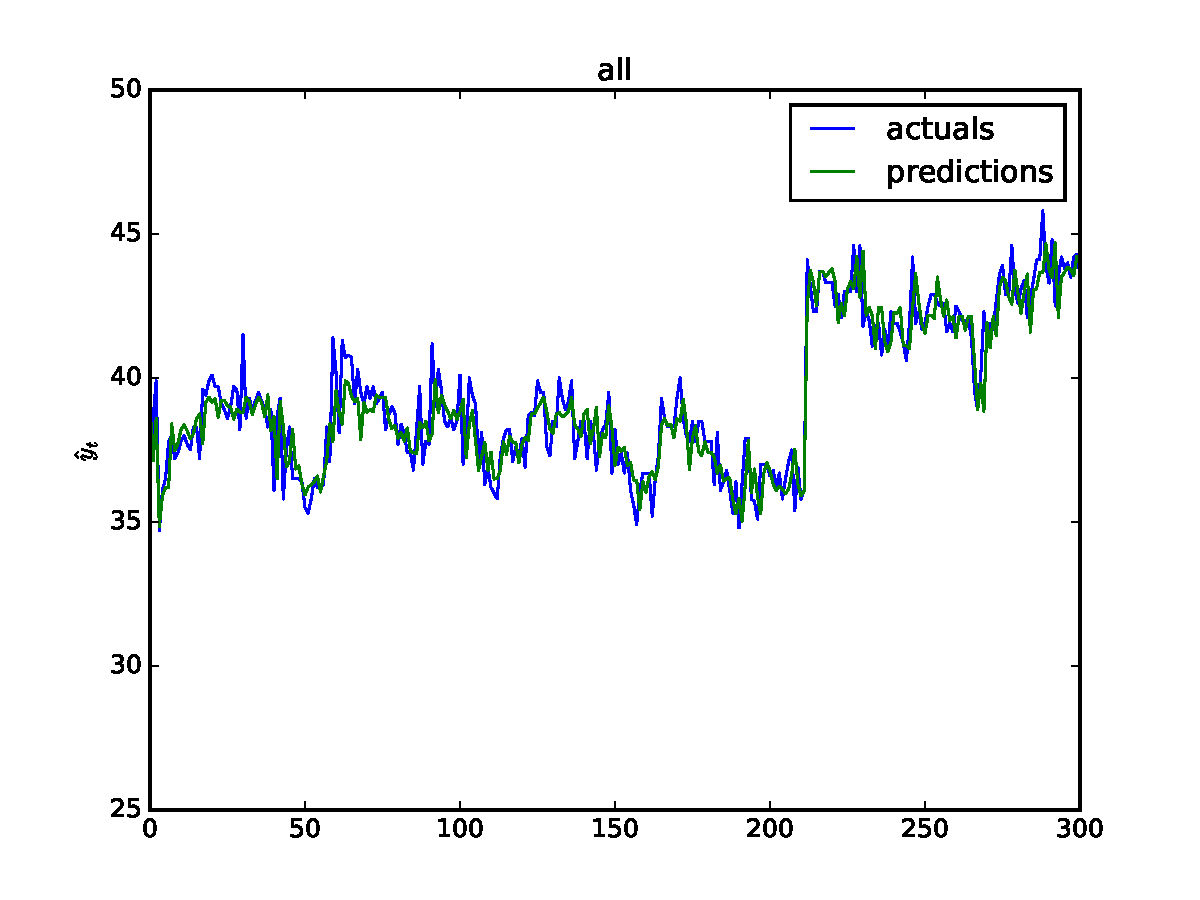
\includegraphics[width=0.9\linewidth]{singleday_all}
\caption{单日数据建模在部分样本上的预测结果。}
\label{fig:singleday_all}
\end{center}
\end{figure}

另外通过XGBoost的plot\_importance函数可以可视化不同特征对于模型的重要性或贡献程度,结果如图\ref{fig:feature_importance}所示。由图可知,当取单日观测数据拟合第二天头均采食量时,各特征重要性排序为:头均采食量>头均产奶量>最高气温。

\begin{figure}
\begin{center}
	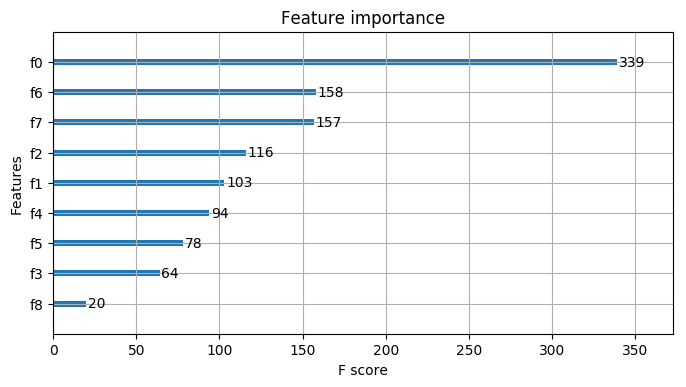
\includegraphics[width=0.9\linewidth]{feature_importance}
\caption{不同特征对XGBoost模型的贡献程度。$f0,f1,f2$分别对应数据样本中的$y_t, m_t, T^h_t$。}
\label{fig:feature_importance}
\end{center}
\end{figure}

模型对历史数据的拟合只能说明模型复杂程度足够高,但不能说明模型对于\uline{未见过的数据样本}具有较强的预测能力,即对于有预测性质的任务,我们更需要关注模型的\emph{泛化能力}。
我们在下一小节做相关分析。

\subsubsection{模拟对未见数据的预测}
\label{predict_singleday}

我们采用交叉验证\footnote{具体地,$k$折交叉验证将所有数据样本随机平均分为$k$组,重复$k$次测试:每次测试用其中$k-1$组数据样本组合成训练集,训练构建得到模型(预测器),并将模型用于剩下的一组数据样本(作为测试集)进行预测,并在测试集上评估相关误差指标。}的方式评估模型的泛化能力,即对历史未见数据的预测能力。


\begin{table}
\caption{单日数据建预测时5折交叉验证的误差。}
\begin{center}
\footnotesize
\begin{tabular}{|c|c|}
\hline
	$\epsilon_{MAE}$ & $R^2$ \\
\hline
 1.202 &  0.728\\
 1.221 &  0.797\\
 1.243 &  0.744 \\
 1.359 &  0.724 \\
 1.430 &  0.560 \\
\hline
\end{tabular}
\end{center}
\label{tab:singleday_predict_all}
\end{table}


表\ref{tab:singleday_predict_all}显示了对所有数据样本做5折交叉验证的结果(交叉验证时不同随机分组会导致不同的结果,表中显示随机挑选某次实验的结果)。
比较表\ref{tab:singleday_predict_all}和\ref{tab:singleday_all},可知预测时的平均$\epsilon_{MAE}=1.291$略高于对照组的$\epsilon_{MAE}$,模型相比于对照组\uline{预测失效}。
虽然在上一节观察到模型拟合历史数据的能力较强,但交叉验证的结果说明模型缺乏泛化能力,这主要由两个可能原因导致:(1)在部分实验中$\epsilon_{MAE}$较高,原因可能是在拆分训练集和测试集时,某些相对难预测的模式的样本被分至测试集但未出现在训练集中(导致模型未能学到这些模式)。
如数据集规模进一步增大,则模型的预测性能应当进一步提升。
(2)仅以单日观测数据作为特征,缺乏对采食量变化模式的刻划能力。我们在第\ref{temporal}节尝试改进措施。



\subsubsection{分牛棚的拟合和预测分析}
\label{predict_singleday_cowshed}

我们进一步分析模型对于不同牛棚的牛群采食量的预测能力。
我们先用所有样本数据训练得到模型去\emph{拟合}各个牛棚的数据,观察模型对于不同牛棚牛群采食量刻划效果的差异,结果如表\ref{tab:regression_multicowshed}所示。

\begin{table}
\caption{不同牛棚头均采食量拟合的误差。}
\begin{center}
\footnotesize
\begin{tabular}{|c|c|c|c|c|}
\hline
	牛棚 & 牛只类型 & $\epsilon_{MAE}$ & 对照组$\epsilon_{MAE}$ &$R^2$ \\
\hline
B1-1N& 头胎 & 0.793 & 0.964 & 0.424 \\
B1-1S& 头胎 & 0.657 & 0.865 & 0.73 \\
B1-3N& 多胎 & 0.756 & 0.751 & 0.475 \\
B1-3S& 头胎 & 0.706 & 0.726 & 0.696 \\
B1-5N& 头胎 & 1.173 & 1.824 & 0.846 \\
B1-5S& 头胎 & 1.375 & 2.806 & 0.919 \\
B1-7N& 头胎 & 1.232 & 1.477 & 0.898 \\
B1-7S& 多胎 & 0.995 & 1.105 & 0.458 \\
B4-1N& 参配 & 1.095 & 1.56 & 0.584 \\
B4-1S& 怀孕 & 0.969 & 1.193 & 0.699 \\
B4-3N& 蹄病 & 1.248 & 1.455 & 0.501 \\
B4-3S& 高产 & 1.39 & 1.743 & 0.564 \\
B4-5N& 多胎 & 0.882 & 1.197 & 0.757 \\
B4-5S& 头胎 & 1.008 & 1.088 & 0.556 \\
B4-7N& 多胎 & 1.071 & 1.192 & 0.664 \\
B4-7S& 头胎 & 0.913 & 0.987 & 0.798 \\
\hline
\end{tabular}
\end{center}
\label{tab:regression_multicowshed}
\end{table}

观察可以发现(1)各牛棚模型拟合平均绝对误差均低于对照组;
(2)不同牛棚拟合的误差有高有低,大致和对照组拟合误差高低趋势一致。
观察(2)说明模型的预测误差主要来自于日头均采食量的较大波动,而模型难以预测这种突然的升、降。
$R^2$值最高的(模型拟合度最高的)几个牛棚为B1-5S、B1-7N、B1-5N、B4-7S、B4-5S($R^2$均高于0.75)。
这些牛棚除B4-5S外,均为“头胎”,其原因可能是“头胎”牛占数据样本中的大多数,使得模型对于该类型牛的采食量模式刻划得较好。而牛只这也说明不同类型牛的采食量模式存在差异。
因而在建模时应当考虑如下权衡:

\emph{问题:建模时应对不同品种、类型(头胎、多胎、参配等)的牛群分别构建模型,还是用同一模型建模,用某些特征来表征这种差异?}

如果数据量充足,且能够提取富有表征能力的特征,则构建统一模型可以达到较好的预测效果(有待未来实验验证)。

但当前训练数据样本有限且特征不够丰富,我们先尝试简化问题进行分牛棚的实验:排除影响模型预测效果的因素,只选取牛只类别为“头胎”的牛棚,单独进行建模。
如此筛选得到约760条数据样本,在所有“头胎”牛棚牛群上进行5折交叉验证,实验结果如表\ref{tab:singleday_first_predict_all}所示。在只考虑“头胎”牛群时,对照组的平均绝对误差$\epsilon_{MAE}$为1.306。观察表格结果可见5折交叉验证的$\epsilon_{MAE}$的平均值1.328高于对照组,且高于不区分牛群时的平均$\epsilon_{MAE}$,说明模型\uline{预测失效}。原因如第\ref{predict_singleday}节所述,主要有二:(1)数据量过小,测试集中存在训练集未涵盖的采食量变化模式,导致模型泛化能力差;(2)模型的输入变量缺乏富有表征力的特征。
其中原因(1)尤为重要,因为如只选择“头胎”牛群,则数据集样本数仅为约760,不到上节全部牛群数据量的一半。

\begin{table}
\caption{单日数据建预测“头胎”牛群时5折交叉验证的误差。}
\begin{center}
\footnotesize
\begin{tabular}{|c|c|}
\hline
	$\epsilon_{MAE}$ & $R^2$ \\
\hline
  1.361  &  0.627 \\
 1.404  &  0.560 \\
 1.231  &  0.750 \\
 1.376  &  0.720 \\
 1.267  &  0.653 \\
\hline
\end{tabular}
\end{center}
\label{tab:singleday_first_predict_all}
\end{table}




\subsection{加入时域信息预测第二天采食量}
\label{temporal}

\begin{figure}
\begin{center}
	\includegraphics[width=0.8\linewidth]{feature_importance_gradient}
\caption{不同特征对XGBoost模型的贡献程度。$f0,f1,f2,f3$分别对应数据样本中的$y_t, m_t, T^h_t, g_{t,k}$。}
\label{fig:feature_importance_gradient}
\end{center}
\end{figure}

本节训练模型使用的数据每条样本格式为:
\begin{equation}
	\langle (y_t, m_t, T^h_t, g_{t,k}), y_{t+1} \rangle
\end{equation}
相比于式\ref{sample}新增了一项$g_{t,k}$,表示从第$t$天开始向前回溯$k$天的采食量的梯度值。
具体地,$g_{t,k}$是用线性回归拟合点集$\{(1, y_{t-k+1}), (2, y_{t-k+2}), \cdots, (k, y_{t})\}$得到直线的斜率。我们希望引入该项来增加刻划时域上头均采食量变化趋势的特征。

我们设定$k=3$(考虑过去3天采食量的梯度),经过数据预处理、缺失值剔除,得到全部数据样本约1700条。实验中XGBoost模型的参数n\_estimators取150,max\_depth取2(参见第\ref{best_para}节)。
在所有数据样本做拟合分析各特征的重要性,结果如图\ref{fig:feature_importance_gradient}所示。
由图可知,当引入时域特征拟合第二天头均采食量时,各特征重要性排序为:头均采食量>头均产奶量>最高气温 $\approx$ 头均采食量时域梯度。


对所有数据样本做5折交叉验证的结果如表\ref{tab:gradient_predict_all}所示。
对照组(用当天头均采食量直接当做第二天头均采食量预测值)的$\epsilon_{MAE}$为1.274。分析表格可见$\epsilon_{MAE}$的平均值1.209低于对照组,说明\uline{预测有效},虽然改进并不显著。

\begin{table}
\caption{加入时域信息预测所有牛群时5折交叉验证的误差。}
\begin{center}
\footnotesize
\begin{tabular}{|c|c|}
\hline
	$\epsilon_{MAE}$ & $R^2$ \\
\hline
1.239 & 0.767 \\
1.193 & 0.772 \\
1.203 & 0.768 \\
1.196 & 0.822 \\
1.215 & 0.706 \\
\hline
\end{tabular}
\end{center}
\label{tab:gradient_predict_all}
\end{table}

我们仿照第\ref{predict_singleday_cowshed}节,剔除其他类别的牛群,仅对“头胎”牛群进行分析,则结果和第\ref{predict_singleday_cowshed}节类似,预测误差1.286高于对照组1.258,且高于不拆分牛群的预测结果(1.209)。数据集样本量不够大是主要原因。


\section{问题描述}
\label{introduction}


泌乳牛的草料采食量会影响其产奶量及其健康状况。
在实际生产中草料需要提前1天时间制备,并且1天后吃剩的草料将不再提供给牛食用,以免变质的草料影响牛的健康情况。因此,饲养员需要提前估计未来1天内牛的自由采食量,并由此上报需要制备的草料量。理想情况下,饲养员希望控制报草量(即实际发放至牛棚的草料量)略大于牛的自由采食量,即一天后草料有剩余但剩余不多,以免不能满足牛的草料需求或者造成草料的浪费。具体地,牧场规定草料剩余量最好不超过当天报草量的5\%。

泌乳牛的草料采食量受到多方面因素的影响,因而每天每牛棚的自由采食量会发生波动。传统生产中饲养员会根据经验对相关因素进行估计判断,以估计每天每牛棚的报草量。
这种方式可能会由于饲养员的经验差异导致或大或小的预测误差,可能会造成饲料不足或饲料浪费的问题。
本工作希望通过对历史采集数据的分析,量化地构建预测泌乳牛采食量的模型,从而给饲养员提供较准确的采食量预测作为参考,辅助饲养员更好地制定报草量。

本文分为以下几个部分:
第\ref{related}节简述关于采食量预测的相关工作情况。
第\ref{analyze}节对采食量预测问题进行分析并形式化地描述问题。
第\ref{dataset}节概述建模所使用的数据以及对数据的处理方式,
第\ref{model}节介绍预测模型,第\ref{evaluation}节展示实验结果并对结果进行分析。
第\ref{futurework}节讨论下一步的工作方向。
\section{采食量预测模型:XGBoost}
\label{model}

\subsection{XGBoost模型简介}

\begin{figure*}
\begin{center}
	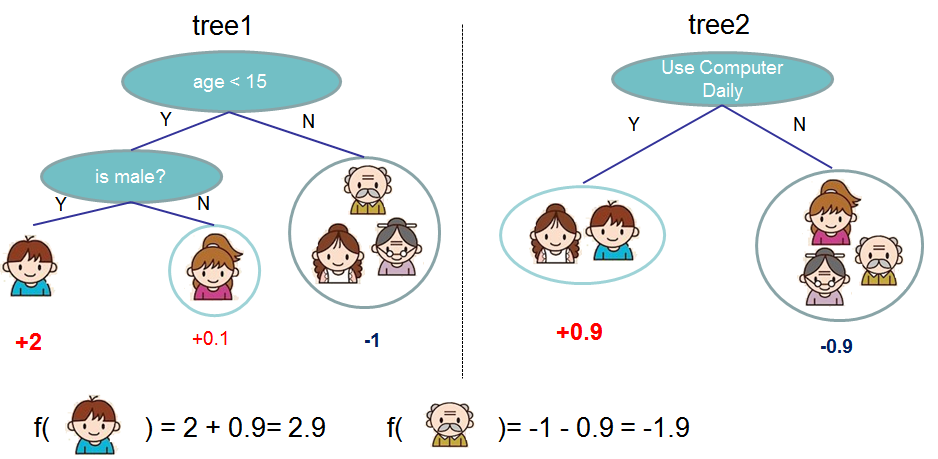
\includegraphics[width=0.8\linewidth]{twocart}
\caption{一个树集成的例子。该包含两棵树的模型解决分类问题,输入变量是每个人的年龄、性别、职业等特征,分类目标是“此人是否喜欢电脑游戏”。树集成将每棵树的输出结果组合起来(本例中为同权重地相加),例如小男孩分类结果为2.9,老爷爷分类结果为-1.9。如果我们设定模型分类阈值为0,则模型认为小男孩喜欢电脑游戏,老爷爷不喜欢。}
\label{twocart}
\end{center}
\end{figure*}


本工作采用XGBoost对采食量进行建模。XGBoost\cite{xgboost_github}是一个专注于梯度提升(gradient boost)算法的机器学习函数库,主要特点是具有优良的学习效果和高效的训练速度。该函数库诞生于2014年2月,最初由陈天奇博士设计、开发,论文\cite{Chen2016XGBoost}具体介绍了其实现原理和细节,演示文稿\cite{xgboost_slides}概述了其主要思想和算法原理。
仅在2015年,在Kaggle\cite{kaggle}竞赛中获胜的29个算法中,有17个使用了XGBoost库。在KDDCup 2015\cite{kddcup2015}竞赛中,排名前十的队伍全部使用了XGBoost库。

XGBoost用于解决监督学习(supervised learning)问题,在监督学习中模型利用训练集进行学习,以通过给定的量$x_i$(多个特征)来预测$y_i$。XGBoost是一种树集成(tree ensemble)模型\footnote{集成(ensemble)模型是一类组合多个性能相对弱的分类器/预测器实现强分类器/预测器的模型。所谓“三个臭皮匠赛过诸葛亮”。},即通过学习得到多棵树,组合起来解决分类问题或回归问题。
图\ref{twocart}展示了一个树集成的例子。

XGBoost优化的目标函数如式\ref{objf}所示:
\begin{equation}
\label{objf}
	obj = \sum_{i=1}^n l(y_i, \hat y_i^{(t)}) + \sum_{i=1}^t \Omega(f_i)
\end{equation}
其中$l(y_i, \hat y_i^{(t)})$表示模型对第$i$个训练集样本的预测误差(误差指标的定义根据问题的不同可以不同。
在回归问题中,均方误差MSE是常用的误差指标),$\Omega(f_i)$表示第$i$棵树的复杂度。
树的复杂度作为正则项,目的是为了控制模型的复杂程度,避免过复杂的模型过度拟合(overfit)训练集而缺乏泛化能力(对未见过样本的预测能力)。

在学习模型参数时,XGBoost采用相加策略:它递推地依次学习出各棵树,每次只增加一棵树,在学习第$t$棵树时,固定前$t-1$棵树不变,而用第$t$棵树去矫正前$t-1$棵树对于样本预测结果的误差(残差学习)。具体地,学习第$t$树时,优化目标函数$obj^{(t)}$为:
\begin{equation}
\label{objf_eachtree}
	obj^{(t)} = \sum_{i=1}^n l(y_i, \hat y_i^{(t-1)} + f_t(x_i)) + \Omega(f_t) + \textrm{常数}
\end{equation}

更多关于XGBoost算法细节请参考XGBoost网站文档、演示文稿和论文\cite{intro_xgboost, xgboost_slides,Chen2016XGBoost}。下面我们讨论使用XGBoost建模时需要重点考虑的模型参数。

\subsection{模型参数设置}

XGBoost的参数详解可参考\cite{xgboost_para}\footnote{XGBoost提供多种编程语言(Python, R, Java, Scala, C++)接口,该文档介绍R语言接口的参数,但其他语言参数与此基本相同。}。

\para{通用参数:}booster指定使用的booster(提升器),默认值为gbtree。使用默认值即可。
如想采用线性模型(采食量预测不适合采用线性模型),可以将其设为gblinear。

\para{Tree Booster参数:}
n\_estimator是树的个数,如需改善过拟合问题,可适当调小n\_estimator。
max\_depth是最大深度限制(模型构造树时可能尚未到此深度即停止扩展),如需改善过拟合问题,可适当调小max\_depth。由于当前预测采食量的模型使用输入变量很少,通常2-3层的树即足够。
eta是学习率,通常使用默认值即可,如需改善过拟合问题,可适当调小eta。
subsample和相关几个参数(colsample\_bytree、colsample\_bylevel)通过对训练集欠采样来避免模型欠拟合。当前预测采食量任务不需要欠采样。

其他参数一般不需要特别设置,使用默认值即可。

\subsection{最优参数搜索}
\label{best_para}

部分参数取值可以通过由在人为给定的参数空间中网格搜索(grid search,即暴力枚举每一种可能的参数组合)确定。
为了避免过拟合,在搜索每组参数组合时,可采用多折交叉验证。
本工作中如不特殊说明,我们采用8折交叉验证。

用Python的scikit-learn库中model\_selection包里的GridSearchCV类\cite{grid_search}可便捷实现利用网格搜索和交叉验证确定最优参数组合。



\section{相关工作概述}
\label{related}

《奶牛营养需要》第7版(NRC 2011)\footnote{该手册有中文版,百度搜索其中文名称即可找到、下载。}\cite{USA2001Nutrient}中,第一章讨论奶牛的干物质采食量(Dry Matter Intake,DMI)。下文引自《奶牛营养需要》中文版原文。

用来预测荷斯坦泌乳牛DMI的方程式为:
\begin{eqnarray}
\label{eqn:dmi}
	 \nonumber DMI (kg/d) =&&(0.372  \times FCM \\
	 \nonumber &&+  0.0968 \times  BW^{0.75}) \\
	&&\times (1 - e^{-0.192 \times(WOL + 3.67)})
\end{eqnarray}
式中FCM=4\%校正乳产量(kg/d);BW=体重(kg);WOL为泌乳周龄;$1-e^{-0.192\times(WOL+3.67)}$为校正泌乳早期DMI下降的校正项。对于泌乳早期的产奶牛来说,方程式1-2预测的结果与Kertz等(1991)所建立方程式的预测结果相一致。最初14周龄泌乳牛干物质采食量以不同方程式预测的比较结果列于图\ref{fig:dmi}。

\begin{figure}
\begin{center}
	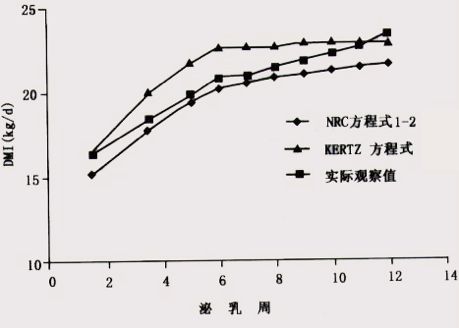
\includegraphics[width=0.9\linewidth]{dmi}
\caption{用方程式\ref{eqn:dmi}和KERTZ等(1991)推荐方程式预测奶牛泌乳早期干物质采食量变化。(图中方程式1-2对应本文中方程式1。)}
\label{fig:dmi}
\end{center}
\end{figure}

方程式\ref{eqn:dmi}的数据全部来自荷斯坦奶牛。目前还没有公开发表关于DMI的数据用于发展或修正目前预测DMI的方程式,以便能用在荷斯坦牛以外其他品种牛上。关于娟姗牛DMI的预测问题,请参见Holter等(1996)的文章。

DMI预测方程式用于经产奶牛可不必进行校正。
在热中温区(5$\sim$20℃)以外,泌乳牛的DMI受到环境的影响。Eastridge等(1998)和Holter等(1997)的研究都表明,当环境温度在20℃以上时,DMI随温度的升高而下降。由于没有足够的数据来确定热中温区以外环境对DMI的影响程度,本版NRC泌乳牛DMI预测方程式(方程式\ref{eqn:dmi})没有考虑温度或湿度校正因子。\documentclass[UTF8,a4paper,10pt, twocolumn]{ctexart}
\usepackage[left=2.50cm, right=2.50cm, top=2.50cm, bottom=2.50cm]{geometry}

% -- text font --
% compile using Xelatex

%\setmainfont{Microsoft YaHei}  % 微软雅黑
%\setmainfont{YouYuan}  % 幼圆    
%\setmainfont{NSimSun}  % 新宋体
%\setmainfont{KaiTi}    % 楷体
%\setmainfont{SimSun}   % 宋体
%\setmainfont{SimHei}   % 黑体

\usepackage{times}
%\usepackage{mathpazo}
%\usepackage{fourier}
%\usepackage{charter}
%\usepackage{helvet}

\usepackage{amsmath, amsfonts, amssymb} % math equations, symbols
\usepackage[english]{babel}
\usepackage{color}      % color content
\usepackage{graphicx}   % import figures
\usepackage{url}        % hyperlinks
\usepackage{bm}         % bold type for equations
\usepackage{multirow}
\usepackage{booktabs}
\usepackage{epstopdf}
\usepackage{epsfig}
\usepackage{algorithm}
\usepackage{algorithmic}
\usepackage{diagbox}


\renewcommand{\algorithmicrequire}{ \textbf{Input:}}     % use Input in the format of Algorithm  
\renewcommand{\algorithmicensure}{ \textbf{Initialize:}} % use Initialize in the format of Algorithm  
\renewcommand{\algorithmicreturn}{ \textbf{Output:}}     % use Output in the format of Algorithm  
\newcommand{\para}[1]{\smallskip\noindent\textbf{#1}}

\newcommand{\wgs}[1]{\textcolor{blue}{\uline{#1}}}

\usepackage{fancyhdr}   % 设置页眉、页脚
%\pagestyle{fancy}
%\lhead{}
%\chead{}
%\rhead{head and foot!!}
%\lfoot{}
%\cfoot{}
%\rfoot{}


\usepackage{hyperref}   % bookmarks
\hypersetup{colorlinks, bookmarks, unicode} % unicode

\graphicspath{{figures/}}


\title{泌乳牛自由采食量预测}
\author{王国赛\thanks{邮箱:wgs14@mails.tsinghua.edu.cn}}
\date{\today}

\begin{document}
    \maketitle
    \thispagestyle{fancy}

\section{问题描述}
\label{introduction}


泌乳牛的草料采食量会影响其产奶量及其健康状况。
在实际生产中草料需要提前1天时间制备,并且1天后吃剩的草料将不再提供给牛食用,以免变质的草料影响牛的健康情况。因此,饲养员需要提前估计未来1天内牛的自由采食量,并由此上报需要制备的草料量。理想情况下,饲养员希望控制报草量(即实际发放至牛棚的草料量)略大于牛的自由采食量,即一天后草料有剩余但剩余不多,以免不能满足牛的草料需求或者造成草料的浪费。具体地,牧场规定草料剩余量最好不超过当天报草量的5\%。

泌乳牛的草料采食量受到多方面因素的影响,因而每天每牛棚的自由采食量会发生波动。传统生产中饲养员会根据经验对相关因素进行估计判断,以估计每天每牛棚的报草量。
这种方式可能会由于饲养员的经验差异导致或大或小的预测误差,可能会造成饲料不足或饲料浪费的问题。
本工作希望通过对历史采集数据的分析,量化地构建预测泌乳牛采食量的模型,从而给饲养员提供较准确的采食量预测作为参考,辅助饲养员更好地制定报草量。

本文分为以下几个部分:
第\ref{related}节简述关于采食量预测的相关工作情况。
第\ref{analyze}节对采食量预测问题进行分析并形式化地描述问题。
第\ref{dataset}节概述建模所使用的数据以及对数据的处理方式,
第\ref{model}节介绍预测模型,第\ref{evaluation}节展示实验结果并对结果进行分析。
第\ref{discussion}节讨论分析依据采食量预测值指定草料投放量面临的问题。
第\ref{futurework}节整理结论并讨论下一步的工作方向。
附录中第\ref{calving_data}节介绍泌乳天数和胎次数据如何获取,第\ref{concat_exp_data}节和第\ref{dwt_exp_data}节是相关实验更具体的结果数据。

\section{相关工作概述}
\label{related}

《奶牛营养需要》第7版(NRC 2011)\footnote{该手册有中文版,百度搜索其中文名称即可找到、下载。}\cite{USA2001Nutrient}中,第一章讨论奶牛的干物质采食量(Dry Matter Intake,DMI)。下文引自《奶牛营养需要》中文版原文。

用来预测荷斯坦泌乳牛DMI的方程式为:
\begin{eqnarray}
\label{eqn:dmi}
	 \nonumber DMI (kg/d) =&&(0.372  \times FCM \\
	 \nonumber &&+  0.0968 \times  BW^{0.75}) \\
	&&\times (1 - e^{-0.192 \times(WOL + 3.67)})
\end{eqnarray}
式中FCM=4\%校正乳产量(kg/d);BW=体重(kg);WOL为泌乳周龄;$1-e^{-0.192\times(WOL+3.67)}$为校正泌乳早期DMI下降的校正项。对于泌乳早期的产奶牛来说,方程式1-2预测的结果与Kertz等(1991)所建立方程式的预测结果相一致。最初14周龄泌乳牛干物质采食量以不同方程式预测的比较结果列于图\ref{fig:dmi}。

\begin{figure}
\begin{center}
	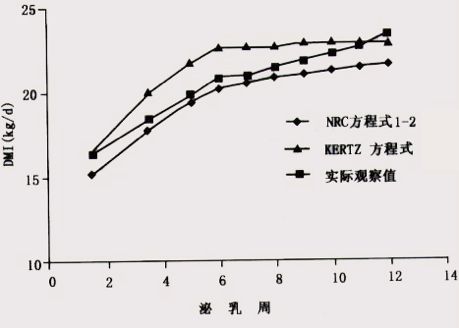
\includegraphics[width=0.9\linewidth]{dmi}
\caption{用方程式\ref{eqn:dmi}和KERTZ等(1991)推荐方程式预测奶牛泌乳早期干物质采食量变化。(图中方程式1-2对应本文中方程式1。)}
\label{fig:dmi}
\end{center}
\end{figure}

方程式\ref{eqn:dmi}的数据全部来自荷斯坦奶牛。目前还没有公开发表关于DMI的数据用于发展或修正目前预测DMI的方程式,以便能用在荷斯坦牛以外其他品种牛上。关于娟姗牛DMI的预测问题,请参见Holter等(1996)的文章。

DMI预测方程式用于经产奶牛可不必进行校正。
在热中温区(5$\sim$20℃)以外,泌乳牛的DMI受到环境的影响。Eastridge等(1998)和Holter等(1997)的研究都表明,当环境温度在20℃以上时,DMI随温度的升高而下降。由于没有足够的数据来确定热中温区以外环境对DMI的影响程度,本版NRC泌乳牛DMI预测方程式(方程式\ref{eqn:dmi})没有考虑温度或湿度校正因子。
\section{问题分析和形式化描述}
\label{analyze}

\subsection{采食量的影响因素}

泌乳牛自由采食量主要受到内部因素和外部因素影响。部分相关因素列举如下:

\para{内部因素:} 

\begin{itemize}
\item
奶牛品种
\item
奶牛泌乳期(胎次,对应不同的泌乳周期,如初产牛、经产牛)
\item
 奶牛泌乳周(或泌乳天数,对应同一泌乳周期中的不同阶段,如高产、中产、低产、干奶)
\item
奶牛体重
\item
奶牛产奶量(产奶浄能)
\item
奶牛运动量
\item
奶牛身心状态(疾病、情绪等)
\end{itemize}

\para{外部因素:} 
\begin{itemize}
\item
饲料特性
\item
温度湿度(热应激)
\item
其他应激(如疫苗注射,受到惊吓等)
\item
其他环境因素(如较宽的槽位可提升采食量)

\end{itemize}

理想情况下,在预测牛的采食量时,模型应将尽可能多的上述因素纳入考虑。
但实际情况中常面临两个问题:(1)数据类别采集不全,(2)数据量积累较少。
问题(1)会制约模型预测目标值采食量的能力,因为未观测/记录到的因素会对采食量带来模型无法预测的波动。
问题(2)会影响模型的精度,因为通常基于机器学习或者数据挖掘技术构建的模型在训练集越大,模型性能会越好,尤其是一些复杂度高的模型如人工神经网络(Artifical Neural Network)深度学习(Deep Learning)等。
故在本工作中我们会取舍地考虑部分因素。详情请见第\ref{dataset}节。

\subsection{以牛舍为建模单位}

生产环境中,牧场对草料的发放以及对剩草量的统计以牛舍为单位,故我们不以单头牛的采食量为预测目标,而是以牛舍中牛群整体的采食量(或者等价的牛舍中头均采食量)为预测目标。通常同牛舍内牛的品种相同,泌乳期相近或相同,泌乳天数相近或相同,故我们在建模时可忽略牛舍内单头牛之间的差异,仅考虑牛群整体的特性(或等价的头均特性)。

\subsection{问题形式化}

生产环境中,每牛舍每天上报一次草量,对应当天中午、晚上和第二天早上三次投喂草料的总草量。

我们记某牛舍第t天上午上报的头均草量(报草量/牛的数量)为$r_{t+1}$\footnote{用$t+1$而不是$t$表示是为了避免在时间先后上引起歧义,可以理解$r_{t+1}$为给牛分配的吃到第$t+1$天的草量。},
接下来的一天内实际头均采食量为$y_{t+1}$。
我们用向量$X_t$表示第$t$天的输入变量。具体地,$X_t$的每一个元素为一个关于牛的或关于环境的观测数据,如第$t$天牛的产奶量等等。

我们希望得到一个预测模型$f$使得
\begin{equation}
	\hat y_{t+1} = f(X_t, X_{t-1}, \cdots, X_{t-w+1}) \approx {y_{t+1}}
\end{equation}
其中$\hat y$表示对$y$变量的预测值,非负整数$w$(window size)表示我们在第$t$天时,回顾历史(含当天)的时间跨度。在最简单的模型中,$w=1$,即
\begin{equation}
	\hat y_{t+1} = f(X_t) \approx {y_{t+1}}
\end{equation}

本项工作中我们主要采用平均绝对误差(Mean Absolute Error,MAE)来衡量模型$f$的预测精度。对于$n$条样本$y_1, y_2 \cdots, y_{n}$和模型对它们的预测值$\hat{y_1}, \hat{y_2}, \cdots, \hat{y_{n}}$,定义平均绝对误差$\epsilon_{MAE}$如下:
\begin{equation}
	\epsilon_{MAE} = \frac 1 n \sum_{i=1}^{n} | \hat{y_i} - y_i | 
\end{equation}








\section{数据集和特征构造}
\label{dataset}

\subsection{数据概览}

本项工作使用的主要数据集取自《剩草量分析表》,包含第三牧场2017年3月5日至7月25日约140天的各牛棚采食情况记录。数据集包含的牛棚列举在表\ref{cowshed}中。数据集记录了16个牛棚每天的\emph{牛头数}\footnote{牛只调群很常见,因此每个牛棚每天的牛群规模可能会有增减。},\emph{报草量},\emph{减草量}\footnote{每天有一次机会可以对上报草量进行增减。例如观察到中午牛食欲不振,则可以适当减少当天至第二天的总草量。减草量也可以为负值,表示适当增加草量。},\emph{剩草量}和\emph{头均产奶量}。通过简单计算可以进一步得到计划头均采食量($r_t =$(报草量-减草量)/牛头数)和实际头均采食量($y_t =$(报草量-减草量-剩草量)/牛头数)。

\begin{table}
\caption{牛棚概览}
\label{cowshed}
\footnotesize
\begin{center}
\begin{tabular}{|c|}
\hline
	\textbf{牛棚}  \\
\hline
    B1-1N  B1-1S  
    B1-3N  B1-3S  \\
    B1-5N  B1-5S  
    B1-7N  B1-7S  \\
    B4-1N  B4-1S  
    B4-3N  B4-3S  \\
    B4-5N  B4-5S  
    B4-7N  B4-7S  \\
\hline
\end{tabular}
\end{center}
\end{table}


\emph{温度、湿度}是影响头均采食量的重要影响参数。温度和湿度数据可从记录历史天气的网站如\cite{weather,tianqi}上抓取获得\footnote{\cite{weather}上可能无湿度信息,\cite{tianqi}上有湿度信息。}。

\emph{泌乳期(胎次)}和\emph{泌乳周}(实际采用的是\emph{泌乳天数})数据可以从牧场管理系统(银香伟业采用阿菲金管理系统)中获取。这两项数据处理的细节请参考附录第\ref{calving_data}节。



\subsection{关于部分未采用数据说明} 
\begin{itemize}
\item 奶牛品种:各牧场主要包含两种奶牛:荷斯坦奶牛和娟姗奶牛(同牛棚同日内牛群属同种)。但当前第三牧场中全部牛只均为荷斯坦奶牛,无娟姗奶牛,故我们不区分牛的品种,对所有数据统一处理。

\item 奶牛体重:我们将牛棚的牛群作为整体分析其头均采食量,故暂时假设各牛棚头均体重相似,不是影响头均采食量的主要因素。

\item 奶牛运动量:当前先假设各牛棚牛群每日运动量相近。如有计步器数据,可将步数信息和采食量做关联性分析。

\item 奶牛身心状况:奶牛身心状况难以量化。目前工作未考虑此类特征。未来工作可考虑通过牧场系统中对牛的检查、治疗等事件记录推断估计出各牛棚的整体健康状态。

\item 饲料特性:各牛棚除新产牛外(?待验证),主要采用同种配方的饲料。本项工作主要针对处高产期的牛的采食量建模,故模型未将饲料相关的数据视作输入变量。

\item 其他应激:当前数据集未包含疫苗注射记录。据技术人员称疫苗注射会令牛产生应激,影响短期内采食量。未来工作可考虑通过牧场系统中对牛的检查、治疗等事件记录推断、量化每天各牛棚可能的应激事件。
\end{itemize}


\subsection{数据预处理和特征构造}

根据《剩草量分析表》中“牛只类型”字段标注,各牛棚在大部分日期内牛属于“高产”,但个别牛棚在部分日期内被标注为“新产”(生产完牛犊后处于泌乳初期的牛?)。在建模前我们将所有标注为“新产”的数据样本剔除掉。
同时部分日期的数据存在缺失值。当前我们采取最简易的缺失值处理手段:将不完整的数据样本剔除掉。


在预测第$t+1$天头均采食量$y_{t+1}$时,本工作尝试多种构建输入变量$X$的方式,主要可分为两类
(1)仅考虑第$t$天的观测情况(头均采食量、头均产奶量、温湿度),和(2)考虑到一段连续日期即$t-w, t-w+1, \cdots, t$天的观测情况,包括头均采食量、头均产奶量、连续w天头均采食量(直接拼接或用小波分解提取系数)等。对时间序列数据的处理请见第\ref{time_series}小节。

我们对于温湿度数据,计算得到THI(Thermal-Humidity Index,温湿度指数)指标作为模型的输入变量,而不是将温度和湿度作为单独的变量输入模型。THI是一个用温度和湿度的综合影响反应热应激水平的指标,它有多种不同的定义/计算方式,最常用的经验公式为:
\begin{equation}
	THI=0.72 \times (Td + Tw) + 40.6
\end{equation}
其中$Td$和$Tw$分别为干湿球温度计读出的干球温度和湿球温度。但由于干湿球温度数据不便于获取,我们在本工作中采用另一种计算THI的公式\cite{thi_cow_wang}:
\begin{equation}
	THI=0.81Td + (0.99Td - 14.3)RH + 46.3
\end{equation}
其中RH(Relative Humidity)为相对湿度。由于每天的温度是个随时间变化的变量,我们在实验中用天气预报给出的当日最高气温来代替公式中的干球温度Td,来表征牛受到热应激的情况。

在附录第\ref{calving_data}节中,我们介绍了各牛只泌乳天数、泌乳期数据的获取。由于我们以牛棚为单位进行建模,我们取各牛棚每天牛群的泌乳天数、泌乳期的\emph{中位数}\footnote{采取中位数而非平均数的动机是避免少量离群点对整体统计指标带来较大偏移。},作为对该日该牛群整体泌乳周期状态的刻划。

\subsubsection{时间序列的处理}
\label{time_series}

我们对多天历史数据采取两种处理方式:直接拼接和提取小波分解的系数作特征。我们分别考虑拼接历史头均采食量的时间序列,或者头均产奶量的时间序列\footnote{我们未同时考虑两个时间序列,因为此两时间序列有一定相关性,且实验发现拼接两个时间序列并未获得更优的测试集误差。},而对其他特征(THI、泌乳天数、胎次)不考虑历史数据。

形式化地,当我们考虑拼接头均采食量时间序列时,每条样本的形式为
\begin{equation}
	\langle (y_{t-w+1}, \cdots, y_t, m_t, T_{t+1}, cd_{t}, cp_{t}), y_{t+1} \rangle
\end{equation}
	其中$y_{t+1}$预测目标,$y_k$为某牛舍第$k$天的实际头均采食量,$m_k$为某牛棚第$k$天的头均产奶量,$T_{k}$为第$k$天的THI值(可借助天气预报获得未来一天的THI值), $cd_{k}$和$cp_{k}$分别为某牛棚第$k$天的泌乳天数和胎次的中位数。
	
类似地,当我们考虑拼接头均产奶量时间序列时,每条样本的形式为
\begin{equation}
	\langle (y_t, m_{t-w+1}, \cdots, m_t, T_{t+1}, cd_{t}, cp_{t}), y_{t+1} \rangle
\end{equation}

另一种处理历史时间序列数据的策略是离散小波分解(Discrete Wavelet Transform,DWT)。小波分解是一种常用的信号处理手段。回顾傅里叶变换将时域的信号通过变换得到了精确的频域信号,但完全丢失了时域信息。小波变换在时域精确测量和频域精确测量间做了折衷。通过小波分解,我们可得到有关信号时域和频域的一些信息。在本文中,我们采用离散小波变换(DWT)。关于小波变换的更多介绍可以参考\cite{vidakovic1994wavelets, valens1999really}和Youtube上搜索“Discrete Wavelet Transform”查询到的相关视频。

离散小波分解的过程可如示意图\ref{dwt}所示。原始信号x(长度为k序列)经过1层小波分解得到长度为k/2的1阶近似和长度为k/2的1阶细节。我们可以继续把1阶近似作为原始信号做1层离散小波分解,得到的长度为k/4的1阶近似和长度为k/4的1阶细节对于信号x而言是2阶近似和2阶细节。以此类推。

\begin{figure}
\begin{center}
	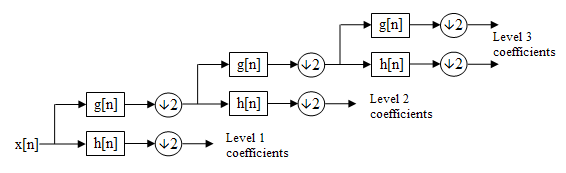
\includegraphics[width=0.95\linewidth]{dwt}
\caption{3层离散小波分解示意图。}
\label{dwt}
\end{center}
\end{figure}

在本工作中,以考虑头均采食量序列为例,我们对于长度为w的序列${y_{t-w+1}, y_{t-w+2}, \cdots, y_t}$做1阶或2阶小波分解,得到$\langle cA, cD\rangle$或$\langle cA', cD', cD\rangle$,并把它们作为特征输入给模型。其中,$cA, cD, cA', cD'$分别为小波分解的1阶近似、细节,2阶近似、细节。因而,以做1阶小波分解为例,每条样本的形式为
\begin{equation}
	\langle (y_t, cA, cD, m_t, T_{t+1}, cd_{t}, cp_{t}), y_{t+1} \rangle
\end{equation}
考虑头均产奶量序列时,对数据的处理与之类似。



数据预处理和特征提取的具体细节请参考代码文件(preprocess.ipynb和model.ipynb)中的文字说明。
不同方式构建模型的性能请见第\ref{evaluation}节。








\section{采食量预测模型:XGBoost}
\label{model}

\subsection{XGBoost模型简介}

\begin{figure*}
\begin{center}
	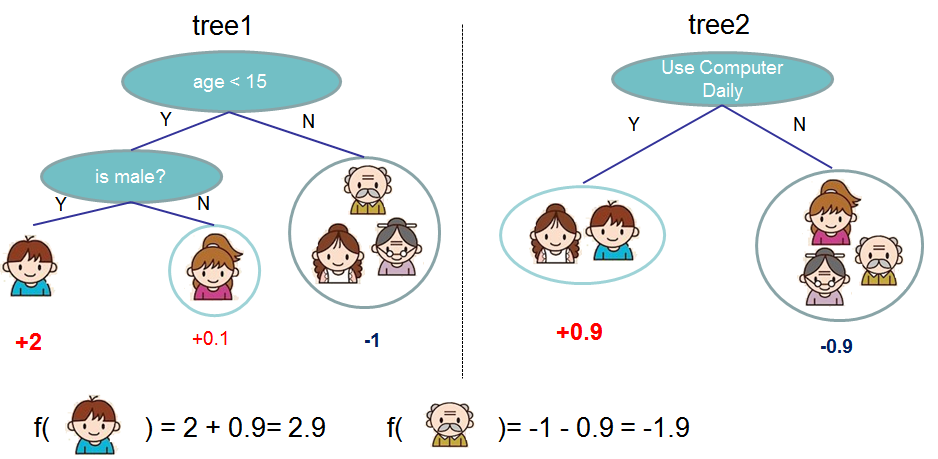
\includegraphics[width=0.8\linewidth]{twocart}
\caption{一个树集成的例子。该包含两棵树的模型解决分类问题,输入变量是每个人的年龄、性别、职业等特征,分类目标是“此人是否喜欢电脑游戏”。树集成将每棵树的输出结果组合起来(本例中为同权重地相加),例如小男孩分类结果为2.9,老爷爷分类结果为-1.9。如果我们设定模型分类阈值为0,则模型认为小男孩喜欢电脑游戏,老爷爷不喜欢。}
\label{twocart}
\end{center}
\end{figure*}


本工作采用XGBoost对采食量进行建模。XGBoost\cite{xgboost_github}是一个专注于梯度提升(gradient boost)算法的机器学习函数库,主要特点是具有优良的学习效果和高效的训练速度。该函数库诞生于2014年2月,最初由陈天奇博士设计、开发,论文\cite{Chen2016XGBoost}具体介绍了其实现原理和细节,演示文稿\cite{xgboost_slides}概述了其主要思想和算法原理。
仅在2015年,在Kaggle\cite{kaggle}竞赛中获胜的29个算法中,有17个使用了XGBoost库。在KDDCup 2015\cite{kddcup2015}竞赛中,排名前十的队伍全部使用了XGBoost库。

XGBoost用于解决监督学习(supervised learning)问题,在监督学习中模型利用训练集进行学习,以通过给定的量$x_i$(多个特征)来预测$y_i$。XGBoost是一种树集成(tree ensemble)模型\footnote{集成(ensemble)模型是一类组合多个性能相对弱的分类器/预测器实现强分类器/预测器的模型。所谓“三个臭皮匠赛过诸葛亮”。},即通过学习得到多棵树,组合起来解决分类问题或回归问题。
图\ref{twocart}展示了一个树集成的例子。

XGBoost优化的目标函数如式\ref{objf}所示:
\begin{equation}
\label{objf}
	obj = \sum_{i=1}^n l(y_i, \hat y_i^{(t)}) + \sum_{i=1}^t \Omega(f_i)
\end{equation}
其中$l(y_i, \hat y_i^{(t)})$表示模型对第$i$个训练集样本的预测误差(误差指标的定义根据问题的不同可以不同。
在回归问题中,均方误差MSE是常用的误差指标),$\Omega(f_i)$表示第$i$棵树的复杂度。
树的复杂度作为正则项,目的是为了控制模型的复杂程度,避免过复杂的模型过度拟合(overfit)训练集而缺乏泛化能力(对未见过样本的预测能力)。

在学习模型参数时,XGBoost采用相加策略:它递推地依次学习出各棵树,每次只增加一棵树,在学习第$t$棵树时,固定前$t-1$棵树不变,而用第$t$棵树去矫正前$t-1$棵树对于样本预测结果的误差(残差学习)。具体地,学习第$t$树时,优化目标函数$obj^{(t)}$为:
\begin{equation}
\label{objf_eachtree}
	obj^{(t)} = \sum_{i=1}^n l(y_i, \hat y_i^{(t-1)} + f_t(x_i)) + \Omega(f_t) + \textrm{常数}
\end{equation}

更多关于XGBoost算法细节请参考XGBoost网站文档、演示文稿和论文\cite{intro_xgboost, xgboost_slides,Chen2016XGBoost}。下面我们讨论使用XGBoost建模时需要重点考虑的模型参数。

\subsection{模型参数设置}

XGBoost的参数详解可参考\cite{xgboost_para}\footnote{XGBoost提供多种编程语言(Python, R, Java, Scala, C++)接口,该文档介绍R语言接口的参数,但其他语言参数与此基本相同。}。

\para{通用参数:}booster指定使用的booster(提升器),默认值为gbtree。使用默认值即可。
如想采用线性模型(采食量预测不适合采用线性模型),可以将其设为gblinear。

\para{Tree Booster参数:}
n\_estimator是树的个数,如需改善过拟合问题,可适当调小n\_estimator。
max\_depth是最大深度限制(模型最终构造的树可能不到此深度),如需改善过拟合问题,可适当调小max\_depth。由于当前预测采食量的模型使用输入变量很少,通常3-4层的树即足够。
eta是学习率,通常使用默认值即可,如需改善过拟合问题,可适当调小eta。
subsample和相关几个参数(colsample\_bytree、colsample\_bylevel)通过对训练集欠采样来避免模型欠拟合。当前预测采食量任务不需要欠采样。

其他参数一般不需要特别设置,使用默认值即可。

\subsection{最优参数搜索}
\label{best_para}

部分参数取值可以通过由在人为给定的参数空间中网格搜索(grid search,即暴力枚举每一种可能的参数组合)确定。
为了避免过拟合,在搜索每组参数组合时,可采用多折交叉验证。
本工作中如不特殊说明,我们采用8折交叉验证。

在实验中可以用Python的scikit-learn库中model\_selection包里的GridSearchCV类\cite{grid_search},它可便捷实现利用网格搜索和交叉验证确定最优参数组合。




\section{实验分析}
\label{evaluation}

\subsection{实验设置}

在实验中我们采用了\emph{对照组},对照组作为比较的基准对象用最简易傻瓜的方式建模预测,具体地,$\hat y_{t+1} = y_t$,即用当天的实际头均采食量直接作为第二天的头均采食量预测值。
对照组的$\epsilon_{MAE}$(基准结果):1.1560。

我们采用交叉验证\footnote{具体地,$k$折交叉验证将所有数据样本随机平均分为$k$组,重复$k$次测试:每次测试用其中$k-1$组数据样本组合成训练集,训练构建得到模型(预测器),并将模型用于剩下的一组数据样本(作为测试集)进行预测,并在测试集上评估相关误差指标。}的方式评估模型的泛化能力,即对历史未见数据的预测能力。以下实验如不另加说明,均为8折交叉验证的结果。

在该节和附录中,我们用表格罗列出使用同种特征时,XGBoost模型选取各种不同参数(包括n\_enumerators和max\_depth)组合的结果。表格中的每一项a/b表示:在某种参数组合下,我们进行8折交叉验证的8次实验中,训练集上的$\epsilon_{MAE}$的平均值为a,测试集上的$\epsilon_{MAE}$的平均值为b。
我们用下划线突出标注每个表格中测试集上表现最优的结果。

%\begin{table}
%\caption{表格部分所用符号注解}
%\label{table_notation}
%\scriptsize
%\begin{center}
%\begin{tabular}{|c|p{5.6cm}|}
%\hline
%\textbf{符号} & \textbf{含义} \\
%\hline
%    THI & Thermal Humidity Index(温度湿度指数)。 \\
%    k & 回顾历史的天数。不加说明时,k=1。  \\
%    cA & 头均采食量时间序列做小波分解的1阶近似。 \\
%    cD & 头均采食量时间序列做小波分解的1阶细节。 \\
%    cA\_milk & 头均产奶量时间序列做小波分解的1阶近似。 \\
%    cD\_milk & 头均产奶量时间序列做小波分解的1阶细节。 \\
%    cA' & 头均采食量时间序列做小波分解的2阶近似。 \\
%    cD' & 头均采食量时间序列做小波分解的2阶细节。 \\
%\hline
%\end{tabular}
%\end{center}
%\end{table}%


\subsection{仅考虑单日数据}

表\ref{table_y_m}、\ref{table_y_m_thi}、\ref{table_y_m_thi_cald}、\ref{table_y_m_thi_cald_calp}是仅考虑当日数据,不考虑历史时序数据(w=1)的预测结果。
其中,表\ref{table_y_m}只考虑了头均采食量和头均产奶量两个特征,\ref{table_y_m_thi}、\ref{table_y_m_thi_cald}、\ref{table_y_m_thi_cald_calp}在该两个特征基础上,依次增加了温湿度指数(THI)、泌乳天数、泌乳期(胎次)特征。

观察表格可以发现:

(1) 就训练集而言,每组特征设置下,随着参数n\_enumerators和max\_depth的不断增大,训练集的误差不断减小。说明越复杂的模型可以越精确地刻划头均采食量的值。但是我们的目的是对未来的头均采食量做预测,我们需要关注模型的泛化性能,因而我们需要关注模型在测试集上的表现。

(2) 就测试集而言,每组特征设置下,在模型复杂度过低(参数n\_enumerators和max\_depth较小)或过高(参数n\_enumerators和max\_depth较大)时,测试集上的误差均相对较大,而在模型复杂度适中时,测试集上的误差相对较小。这说明过高的模型复杂度会导致过拟合现象,引起测试集上误差增大。我们可以通过比较测试集上的误差推断在某种特征设置下,什么是最合适的参数组合。

(3) 随着特征的不断丰富,测试集上的最小误差不断下降(由表\ref{table_y_m}中的1.168下降至\ref{table_y_m_thi_cald_calp}中的1.1014,说明增加的特征有助于模型更精准地刻划第二天的头均采食量。


\begin{table*}
\caption{头均采食量+头均产奶量}
\label{table_y_m}
\scriptsize
\begin{center}
	\begin{tabular}{|c|c|c|c|c|c|c|}
\hline
& \multicolumn{6}{|c|}{n\_enumerators} \\ \cline{2-7}
max\_depth & 75 & 100 & 150 & 200 & 250 & 300\\
\hline
1 & 1.1352/1.1788 & 1.1218/1.1722 & 1.1129/1.1691 & 1.1085/1.1686 & 1.1055/\wgs{1.168} & 1.1035/1.1681 \\
2 & 1.0972/1.1678 & 1.0863/1.1683 & 1.0692/1.1702 & 1.055/1.1718 & 1.0417/1.1749 & 1.0298/1.1776 \\
3 & 1.0627/1.1684 & 1.0451/1.1715 & 1.0161/1.1739 & 0.9879/1.18 & 0.9626/1.1864 & 0.9407/1.1947 \\
\hline
	\end{tabular}
\end{center}
\end{table*}%


\begin{table*}
\caption{头均采食量+头均产奶量+THI}
\label{table_y_m_thi}
\scriptsize
\begin{center}
	\begin{tabular}{|c|c|c|c|c|c|c|}
\hline
& \multicolumn{6}{|c|}{n\_enumerators} \\ \cline{2-7}
max\_depth & 75 & 100 & 150 & 200 & 250 & 300\\
\hline
1 & 1.1354/1.1794 & 1.1217/1.1716 & 1.1105/1.1684 & 1.1054/1.1678 & 1.1016/1.1671 & 1.0985/1.166 \\
2 & 1.0812/1.1526 & 1.0672/1.1498 & 1.0431/1.1452 & 1.0227/1.1426 & 1.0053/1.1397 & 0.9907/1.1388 \\
3 & 1.0284/1.1404 & 1.0019/1.1336 & 0.9587/1.1291 & 0.9239/\wgs{1.1277} & 0.894/1.1325 & 0.8668/1.1347 \\
4 & 0.9742/1.1415 & 0.9344/1.1329 & 0.8714/1.1288 & 0.8182/1.1311 & 0.7711/1.1366 & 0.7292/1.1423 \\
\hline
	\end{tabular}
\end{center}
\end{table*}%


\begin{table*}
\caption{头均采食量+头均产奶量+THI+泌乳天数}
\label{table_y_m_thi_cald}
\scriptsize
\begin{center}
	\begin{tabular}{|c|c|c|c|c|c|c|}
\hline
& \multicolumn{6}{|c|}{n\_enumerators} \\ \cline{2-7}
max\_depth & 75 & 100 & 150 & 200 & 250 & 300\\
\hline
1 & 1.1275/1.1739 & 1.1066/1.1591 & 1.0867/1.1474 & 1.0767/1.1431 & 1.0717/1.1419 & 1.0682/1.1416 \\
2 & 1.0512/1.1307 & 1.0335/1.1262 & 1.0078/1.124 & 0.9868/1.1187 & 0.9682/1.1187 & 0.9526/1.1195 \\
3 & 0.9884/1.1195 & 0.9595/1.1142 & 0.9116/1.1095 & 0.8733/1.1108 & 0.8391/1.1144 & 0.8088/1.1166 \\
4 & 0.9203/1.1086 & 0.8784/\wgs{1.1029} & 0.8068/1.1067 & 0.7481/1.1102 & 0.6973/1.1184 & 0.6521/1.1263 \\
5 & 0.8504/1.1032 & 0.79/1.1093 & 0.6967/1.12 & 0.6172/1.1312 & 0.5508/1.1443 & 0.4921/1.1507 \\
\hline
	\end{tabular}
\end{center}
\end{table*}%

\begin{table*}
\caption{头均采食量+头均产奶量+THI+泌乳天数+胎次}
\label{table_y_m_thi_cald_calp}
\scriptsize
\begin{center}
	\begin{tabular}{|c|c|c|c|c|c|c|}
\hline
& \multicolumn{6}{|c|}{n\_enumerators} \\ \cline{2-7}
max\_depth & 75 & 100 & 150 & 200 & 250 & 300\\
\hline
1 & 1.1266/1.1745 & 1.1066/1.1605 & 1.0873/1.1501 & 1.0775/1.1458 & 1.0724/1.1443 & 1.0686/1.1439 \\
2 & 1.0507/1.1341 & 1.0328/1.1273 & 1.0069/1.1233 & 0.9859/1.1207 & 0.9667/1.1167 & 0.9513/1.1158 \\
3 & 0.9867/1.1205 & 0.957/1.1134 & 0.9102/1.1103 & 0.8706/1.1094 & 0.8381/1.1092 & 0.8069/1.1126 \\
4 & 0.9192/1.106 & 0.875/\wgs{1.1014} & 0.8037/1.1029 & 0.7431/1.1052 & 0.6911/1.1108 & 0.6455/1.1137 \\
5 & 0.8435/1.1049 & 0.7807/1.1061 & 0.6858/1.1129 & 0.6047/1.1216 & 0.5376/1.1314 & 0.4801/1.141 \\
\hline
	\end{tabular}
\end{center}
\end{table*}%


\subsection{直接拼接多日时序数据}
\label{multiday_concat}

\begin{table}
\caption{直接拼接多日时序数据,测试集的$\epsilon_{MAE}$}
\label{table_total_concat}
\scriptsize
\begin{center}
	\begin{tabular}{|c|c|c|c|c|}
\hline
& \multicolumn{4}{|c|}{时间窗口大小 $w$} \\ \cline{2-5}
考虑时间序列的特征 & 2 & 3 & 4 & 5\\
\hline
头均采食量 & 1.1028 & 1.0993 & 1.091 & 1.0976 \\
头均产奶量 & 1.0979 & 1.0882 & \wgs{1.087} & 1.1007 \\
\hline
	\end{tabular}
\end{center}
\end{table}

本节和下一节我们考虑时间窗口大小w>1的情况,即我们在预测第二天的头均采食量时,除了考虑当天外,也考虑过去若干天的历史数据。在本节中,我们对多天历史数据采取直接拼接的处理方式。

表\ref{table_total_concat}概括列出了拼接不同时间序列时,测试集上的最优误差。具体实验结果请见附录第\ref{concat_exp_data}节中的表\ref{table_y2_m_thi_cald_calp}、\ref{table_y3_m_thi_cald_calp}、\ref{table_y4_m_thi_cald_calp}、\ref{table_y5_m_thi_cald_calp}和表\ref{table_y_m2_thi_cald_calp}、\ref{table_y_m3_thi_cald_calp}、\ref{table_y_m4_thi_cald_calp}、\ref{table_y_m5_thi_cald_calp}。


观察各表格可见考虑头均采食量和考虑头均产奶量历史数据得到的最优$\epsilon_{MAE}$比较接近(相差在均在0.012kg以内),在多个w取值(w=2,3,4)下,考虑头均产奶量历史数据实验得到的预测误差更小,且w取不同值时,测试集上最优的误差(1.087)在w=4,考虑头均产奶量历史数据时得到。




%
% Using wavelet decomposition
%
\subsection{小波分解考虑多日时序数据}
\label{multiday_dwt}

\begin{table}
\caption{一阶小波分解处理多日时序数据,测试集的$\epsilon_{MAE}$}
\label{table_total_dwt}
\scriptsize
\begin{center}
	\begin{tabular}{|c|c|c|c|c|}
\hline
& \multicolumn{4}{|c|}{时间窗口大小 $w$} \\ \cline{2-5}
考虑时间序列的特征 & 2 & 4 & 4(二阶) & 6\\
\hline
头均采食量 & 1.0851 & 1.0807 & 1.0858 & 1.0982 \\
头均产奶量 & 1.1016 & \wgs{1.0788} & 1.084 & 1.10939 \\
\hline
	\end{tabular}
\end{center}
\end{table}


本节我们同样考虑时间窗口大小w>1的情况。
本节中我们对多天头均采食量或头均产奶量历史数据的时间序列采取小波分解的方式提取特征。

表\ref{table_total_dwt}概括列出了对不同时间序列做不同处理时,测试集上的最优误差。具体实验结果请见附录第\ref{dwt_exp_data}节中的表\ref{table_wavelet_y2_m}、\ref{table_wavelet_y4_m}、\ref{table_wavelet_y4_2_m}、\ref{table_wavelet_y6_m}和表\ref{table_wavelet_y_m2}、\ref{table_wavelet_y_m4}、\ref{table_wavelet_y_m4_2}、\ref{table_wavelet_y_m6}。

观察各表格可见,与第\ref{multiday_concat}类似,考虑头均采食量和考虑头均产奶量历史数据得到的最优$\epsilon_{MAE}$比较接近(相差均在0.017kg以内),且在不同w取值下,两种考虑不同历史数据的方式的结果各有优劣,不存在绝对更优的一种历史数据处理方式。

测试集上最优的$\epsilon_{MAC}$(1.0788)在w=4,进行1层小波分解,考虑头均产奶量历史数据时得到。这也是\uline{所有实验中得到的最优结果}。和对照组的$\epsilon_{MAC}$(1.1560)相比,模型将预测头均采食量的平均绝对误差降低了$1.1560 - 1.0788=0.0772$。这意味着,XGBoost模型的预测和最简单的预测(用当天的头均采食量作为第二天头均采食量的预测值)相比,头均采食量的平均绝对误差下降了7.7\%千克。



\subsection{特征的重要程度}

图\ref{feature_importance}显示了最优结果($\epsilon_{MAE} = 1.0788$)对应的参数配置下(w=4,头均产奶量时间序列一层小波分解,max\_depth=4,n\_enumerator=100),一次交叉验证实验中,训练出的XGBoost模型调用函数plot\_importance\footnote{参见XGBoost的API文档:\url{http://xgboost.readthedocs.io/en/latest/python/python\_api.html\#module-xgboost.plotting}。}得到的各特征的权重。其中各编号对应的特征列举在表\ref{feature_desc}中。由于做8折交叉验证时训练出的8个模型得到的特征重要程度排序略有不同,我们综合考虑8次实验得到的8个特征排序,将特征按重要程度大致分为如下三组:076/214/538,其中权重最高的三个特征(076)为头均采食量、泌乳天数和THI,次高的三个特征(214)为:头均产奶量、小波分解的1阶近似和细节中各一个分量,最低的三个特征(538)为:小波分解的1阶近似和细节中各一个分量和胎次。

\begin{figure}
\begin{center}
	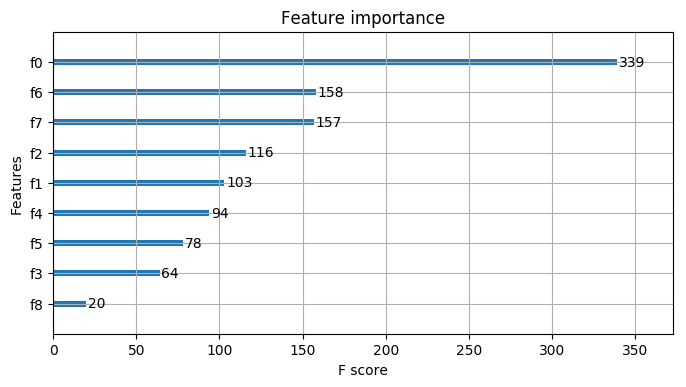
\includegraphics[width=0.95\linewidth]{feature_importance}
\caption{表\ref{table_total_concat}中最优结果对应的参数配置下,某次交叉验证中构建的回归树里各特征的权重。}
\label{feature_importance}
\end{center}
\end{figure}


\begin{table}
\caption{图\ref{feature_importance}中各编号对应的特征}
\label{feature_desc}
\footnotesize
\begin{center}
\begin{tabular}{|c|c|}
\hline
	特征编号	& 特征 \\
\hline
	f0 & $y_t$:头均采食量 \\
	f1 & $m_t$:头均产奶量\\
	f2, f3 & cA:小波分解1阶近似 \\
	f4, f5 & cD:小波分解1阶细节\\
	f6 & $T_{t+1}$:THI \\
	f7 & $cd_t$:泌乳天数 \\
	f8 & $cp_t$:胎次 \\
\hline
\end{tabular}
\end{center}
\end{table}%
















\section{小结与下一步工作方向}
\label{futurework}

\subsection{实验结论整理}

xgboost模型对历史数据的拟合能力很强。但是头均采食量预测任务要求模型具有较好的泛化性能(对未见过数据样本的预测能力)。因此实验需要考察拆分训练集、测试集,交叉验证的结果。本工作未划分验证集。未来工作可考虑划分训练集、测试集、验证集。


通过实验我们发现使用单日观测数据对第二天头均采食量进行预测的效果较差,当引入时域信息(用最近几日头均采食量或产奶量的时序特征)后,模型的预测性能能够提升,但提升不够显著。我们在不同实验中得到的最优结果1.0788相对于对照组1.1560有0.077的提升,来自于除基本特征外,引入近4天头均产奶量历史数据1阶小波分解的系数作为特征构建的模型。

以得到最优预测结果的模型为例,通过对各特征的重要性进行分析,可知对xgboost模型预测第二天头均采食量最重要的特征是当天的头均采食量,泌乳天数和THI,其次最近4天头均产奶量时间序列小波分解得到的1阶近似和1阶细节,泌乳期(胎次)的权重最低。


当前基于数据的利用XGBoost模型建模、预测头均采食量的方法制定备草量仍然具有一定的采食不足或剩草过多的风险。为了进一步优化草量投放量,我们可以从多个角度进行探索,包括:饲养员的角度,模型预测能力的角度,草料制备策略的角度和草料投放策略的角度。在探索各个角度的优化策略的同时,不能忽略了相关手段可能带来的额外成本。

\subsection{未来工作方向}

接下来工作主要分为三块:数据集扩充,特征扩充,特征工程。

\para{数据集扩充:}扩大数据集样本量,积累更多数据。数据积累需要时间。如历史上(2017年3月以前)有各牛棚新增的采食量(或剩草量)数据,也可合并进入当前数据集。且在未来如有可能可在牛棚中增加部署传感器,例如温湿度传感器等等。当前工作采用的数据集覆盖时间段为3月至7月,此段期间THI指数整体稳步上升(由稳步上升的温度主导),如能扩大数据集的时间段至覆盖全年,则可以使训练集学习到更多THI趋势(平稳、下降)下头均采食量的变化规律。

\para{特征扩充:}未来工作可以将其他有记录的应激情况(如牛棚疫苗注射记录)纳入分析。如有可能,可另外增加牛的运动量数据(如计步器采集数据)。

\para{特征工程和模型:}尝试各种特征提取、变换方式以提升模型的预测性能,或者在数据集足够大的情况下尝试神经网络模型。

\begin{appendix}

\section{泌乳天数、泌乳期数据的获取和整理}
\label{calving_data}

牧场管理系统中泌乳天数和泌乳期只有各牛只当天(访问软件进行查询的日期)的数据,而没有历史上每一天的数据。为了将这两项数据作为特征,我们需要解决两个问题:(1) 确定每头牛在历史上每天处于哪一个牛棚(因为我们以牛棚为单位进行建模);(2)确定每头牛在历史上每天的泌乳天数和泌乳期。
	
为了解决问题(1),我们可以借助牧场管理系统中的“改变组别”(组别和牛棚有确定的映射关系)事件记录,来反推出历史上每一天各牛只所在牛群的情况。具体地,获得管理系统访问权限后,进入“动物”——“事件报告”——“事件列表”,即可访问一段时期内,所有被系统记录的牛只事件(如兽医治疗事件、繁育操作事件等),包括改变组别事件。组别改变事件的格式可抽象为$\langle id, t, g_1, g_2\rangle$,其中$id$为牛的编号,$t$为日期,$g_1$为改变前组别,$g_2$为改变后组别。对于每一头牛,我们整理出它的所有改变组别的事件序列(按日期排序),从而可以推断得到一定时间范围内,该牛只每天所处的牛棚(组别和牛棚的映射关系可从系统中的动物报告中抓取解析得到)。

为了解决问题(2),我们可以访问管理系统中的“动物”——“动物报告”板块。如果板块中已存在的“泌乳牛”等报告缺乏我们关系的某些字段(如泌乳期),则我们可以仿照“泌乳牛”报告,新建一个报告,根据需要(定制化报告所需包含的字段)构造出包含所有牛只在\emph{当前日期}的泌乳天数、泌乳期(胎次)、组别数据的报告。由此我们可获得牛只编号和当天(访问软件进行查询的日期)泌乳天数和泌乳期,从而可以追溯历史反推出过去每一天,每头牛的泌乳天数和泌乳期。当推断泌乳天数降至负整数后,我们有两种可能的应对措施:忽略该头牛在上个泌乳周期中的所有泌乳天数、胎次数据,和直接/间接查询或估计该头牛的上一个泌乳周期开始的日期。在本工作中由于时间跨度不是很长(约4-5个月),我们为了简化数据预处理工作,采取第一个策略。
	


\section{直接拼接实验结果记录}
\label{concat_exp_data}

考虑头均采食量时间序列数据的实验结果记录请见表\ref{table_y2_m_thi_cald_calp}、\ref{table_y3_m_thi_cald_calp}、\ref{table_y4_m_thi_cald_calp}、\ref{table_y5_m_thi_cald_calp}。
考虑头均产奶量时间序列数据的实验结果记录请见表\ref{table_y_m2_thi_cald_calp}、\ref{table_y_m3_thi_cald_calp}、\ref{table_y_m4_thi_cald_calp}、\ref{table_y_m5_thi_cald_calp}。

各表格标题中的数字下标代表时间窗口w的大小。例如“头均采食量$_3$”表示我们考虑时间序列$\{ y_{t-2}, y_{t-1}, y_t \}$。

\begin{table*}
\caption{(直接拼接)头均采食量$_2$+头均产奶量+THI+泌乳天数+胎次}
\label{table_y2_m_thi_cald_calp}
\scriptsize
\begin{center}
	\begin{tabular}{|c|c|c|c|c|c|c|}
\hline
& \multicolumn{6}{|c|}{n\_enumerators} \\ \cline{2-7}
max\_depth & 75 & 100 & 150 & 200 & 250 & 300\\
\hline
1 & 1.0762/1.1387 & 1.0587/1.1249 & 1.0436/1.1174 & 1.0359/1.1152 & 1.0309/1.1137 & 1.0273/1.1134 \\
2 & 1.0138/1.1089 & 0.997/1.1065 & 0.9716/1.1048 & 0.9498/1.1045 & 0.9312/1.1057 & 0.9149/1.108 \\
3 & 0.9544/1.107 & 0.9256/1.1038 & 0.8773/1.1076 & 0.8379/1.1113 & 0.8014/1.1173 & 0.7686/1.1187 \\
4 & 0.8883/1.1043 & 0.8439/\wgs{1.1028} & 0.7687/1.1084 & 0.7016/1.1163 & 0.6443/1.1237 & 0.5933/1.1319 \\
5 & 0.8115/1.105 & 0.7465/1.1103 & 0.6364/1.1234 & 0.5528/1.136 & 0.4813/1.146 & 0.4234/1.1539 \\
\hline
	\end{tabular}
\end{center}
\end{table*}%



\begin{table*}
\caption{(直接拼接)头均采食量$_3$+头均产奶量+THI+泌乳天数+胎次}
\label{table_y3_m_thi_cald_calp}
\scriptsize
\begin{center}
	\begin{tabular}{|c|c|c|c|c|c|c|}
\hline
& \multicolumn{6}{|c|}{n\_enumerators} \\ \cline{2-7}
max\_depth & 75 & 100 & 150 & 200 & 250 & 300\\
\hline
1 & 1.0715/1.1354 & 1.0536/1.1236 & 1.0385/1.1173 & 1.0294/1.1124 & 1.0234/1.1104 & 1.0193/1.1095 \\
2 & 1.0061/1.1084 & 0.9891/1.1048 & 0.9621/1.1002 & 0.9391/\wgs{1.0993} & 0.9193/1.0995 & 0.9016/1.0994 \\
3 & 0.9447/1.1117 & 0.9139/1.1077 & 0.8611/1.1024 & 0.8163/1.1019 & 0.7757/1.1072 & 0.7385/1.1094 \\
4 & 0.8726/1.1061 & 0.8239/1.1084 & 0.7422/1.1122 & 0.6721/1.1196 & 0.6115/1.126 & 0.557/1.1355 \\
\hline
	\end{tabular}
\end{center}
\end{table*}%

\begin{table*}
\caption{(直接拼接)头均采食量$_4$+头均产奶量+THI+泌乳天数+胎次}
\label{table_y4_m_thi_cald_calp}
\scriptsize
\begin{center}
	\begin{tabular}{|c|c|c|c|c|c|c|}
\hline
& \multicolumn{6}{|c|}{n\_enumerators} \\ \cline{2-7}
max\_depth & 75 & 100 & 150 & 200 & 250 & 300\\
\hline
1 & 1.065/1.1274 & 1.0459/1.1149 & 1.0296/1.109 & 1.0204/1.1069 & 1.0146/1.1056 & 1.0105/1.1053 \\
2 & 1.0007/1.0959 & 0.9821/1.0929 & 0.9537/\wgs{1.091} & 0.9316/1.094 & 0.9102/1.0948 & 0.8922/1.0955 \\
3 & 0.9393/1.0976 & 0.9066/1.0972 & 0.8532/1.101 & 0.809/1.1048 & 0.7712/1.1068 & 0.7329/1.1133 \\
4 & 0.8673/1.0947 & 0.8206/1.0934 & 0.733/1.098 & 0.6625/1.1093 & 0.5999/1.1189 & 0.5435/1.1291 \\
\hline
	\end{tabular}
\end{center}
\end{table*}%

\begin{table*}
\caption{(直接拼接)头均采食量$_5$+头均产奶量+THI+泌乳天数+胎次}
\label{table_y5_m_thi_cald_calp}
\scriptsize
\begin{center}
	\begin{tabular}{|c|c|c|c|c|c|c|}
\hline
& \multicolumn{6}{|c|}{n\_enumerators} \\ \cline{2-7}
max\_depth & 75 & 100 & 150 & 200 & 250 & 300\\
\hline
1 & 1.064/1.1296 & 1.0452/1.1174 & 1.0282/1.1099 & 1.0193/1.1086 & 1.0131/1.107 & 1.0088/1.1059 \\
2 & 0.9981/1.1052 & 0.9805/1.1016 & 0.9525/1.1013 & 0.9285/1.1049 & 0.9073/1.1044 & 0.8873/1.104 \\
3 & 0.9374/1.1031 & 0.9048/1.1011 & 0.8503/1.1006 & 0.8031/\wgs{1.0976} & 0.7598/1.1004 & 0.7217/1.1045 \\
4 & 0.8631/1.1058 & 0.8168/1.1062 & 0.7298/1.1127 & 0.6534/1.1196 & 0.5888/1.1273 & 0.5301/1.1375 \\
\hline
	\end{tabular}
\end{center}
\end{table*}%

%\subsection{考虑多天头均产奶量时间序列}


\begin{table*}
\caption{(直接拼接)头均采食量+头均产奶量$_2$+THI+泌乳天数+胎次}
\label{table_y_m2_thi_cald_calp}
\scriptsize
\begin{center}
	\begin{tabular}{|c|c|c|c|c|c|c|}
\hline
& \multicolumn{6}{|c|}{n\_enumerators} \\ \cline{2-7}
max\_depth & 75 & 100 & 150 & 200 & 250 & 300\\
\hline
1 & 1.115/1.1611 & 1.0948/1.1465 & 1.076/1.1349 & 1.0661/1.1299 & 1.0605/1.1278 & 1.0569/1.1269 \\
2 & 1.0418/1.1236 & 1.0227/1.1174 & 0.9952/1.1126 & 0.9728/1.1095 & 0.9528/1.1087 & 0.9356/1.1084 \\
3 & 0.975/1.1136 & 0.9432/1.1097 & 0.891/1.1078 & 0.8505/1.1102 & 0.815/1.1148 & 0.7827/1.1169 \\
4 & 0.9019/1.1034 & 0.8528/\wgs{1.0979} & 0.7804/1.1015 & 0.7202/1.1076 & 0.6675/1.1181 & 0.6207/1.1216 \\
5 & 0.8135/1.1028 & 0.7529/1.1057 & 0.6534/1.115 & 0.5708/1.1271 & 0.5009/1.1355 & 0.4446/1.1423 \\
\hline
	\end{tabular}
\end{center}
\end{table*}%


\begin{table*}
\caption{(直接拼接)头均采食量+头均产奶量$_3$+THI+泌乳天数+胎次}
\label{table_y_m3_thi_cald_calp}
\scriptsize
\begin{center}
	\begin{tabular}{|c|c|c|c|c|c|c|}
\hline
& \multicolumn{6}{|c|}{n\_enumerators} \\ \cline{2-7}
max\_depth & 75 & 100 & 150 & 200 & 250 & 300\\
\hline
1 & 1.1098/1.158 & 1.0889/1.1419 & 1.0695/1.1292 & 1.0594/1.1235 & 1.0533/1.1211 & 1.0489/1.12 \\
2 & 1.0286/1.1118 & 1.0094/1.1072 & 0.9817/1.1073 & 0.9583/1.1022 & 0.9391/1.101 & 0.9213/1.1008 \\
3 & 0.9635/1.1028 & 0.9321/1.1005 & 0.8807/1.0986 & 0.8368/1.1026 & 0.7973/1.1064 & 0.7623/1.108 \\
4 & 0.8907/\wgs{1.0882} & 0.8416/1.0892 & 0.7612/1.0952 & 0.6962/1.1024 & 0.6387/1.1106 & 0.5891/1.1153 \\
5 & 0.8104/1.0954 & 0.7426/1.0985 & 0.6281/1.1084 & 0.5388/1.1162 & 0.4678/1.1254 & 0.4067/1.132 \\
\hline
	\end{tabular}
\end{center}
\end{table*}%


\begin{table*}
\caption{(直接拼接)头均采食量+头均产奶量$_4$+THI+泌乳天数+胎次}
\label{table_y_m4_thi_cald_calp}
\scriptsize
\begin{center}
	\begin{tabular}{|c|c|c|c|c|c|c|}
\hline
& \multicolumn{6}{|c|}{n\_enumerators} \\ \cline{2-7}
max\_depth & 75 & 100 & 150 & 200 & 250 & 300\\
\hline
1 & 1.1049/1.1497 & 1.0835/1.134 & 1.0633/1.1221 & 1.0531/1.1171 & 1.0468/1.1137 & 1.0422/1.1128 \\
2 & 1.0268/1.1048 & 1.0082/1.0992 & 0.978/1.0931 & 0.9544/1.0895 & 0.9335/1.0881 & 0.9147/1.0883 \\
3 & 0.9616/1.0947 & 0.9306/1.0915 & 0.8767/\wgs{1.087} & 0.8301/1.091 & 0.7895/1.0959 & 0.7525/1.1041 \\
4 & 0.8906/1.093 & 0.8419/1.0906 & 0.7561/1.0976 & 0.6837/1.107 & 0.6235/1.1143 & 0.5713/1.1207 \\
\hline
	\end{tabular}
\end{center}
\end{table*}%


\begin{table*}
\caption{(直接拼接)头均采食量+头均产奶量$_5$+THI+泌乳天数+胎次}
\label{table_y_m5_thi_cald_calp}
\scriptsize
\begin{center}
	\begin{tabular}{|c|c|c|c|c|c|c|}
\hline
& \multicolumn{6}{|c|}{n\_enumerators} \\ \cline{2-7}
max\_depth & 75 & 100 & 150 & 200 & 250 & 300\\
\hline
1 & 1.1064/1.1528 & 1.0854/1.1371 & 1.0648/1.1263 & 1.0538/1.1228 & 1.0468/1.1209 & 1.0417/1.1201 \\
2 & 1.0294/1.1164 & 1.0099/1.1146 & 0.9775/1.1099 & 0.951/1.1084 & 0.9284/1.1079 & 0.9087/1.1085 \\
3 & 0.9643/1.1072 & 0.9282/1.1036 & 0.8703/1.1053 & 0.8207/1.1053 & 0.7791/1.1084 & 0.7425/1.1158 \\
4 & 0.8881/1.1028 & 0.8391/1.1028 & 0.7488/1.1055 & 0.6757/1.1168 & 0.6141/1.1225 & 0.5615/1.1324 \\
5 & 0.8017/\wgs{1.1007} & 0.7281/1.106 & 0.6077/1.1168 & 0.5172/1.1312 & 0.4433/1.1453 & 0.3801/1.1534 \\
\hline
	\end{tabular}
\end{center}
\end{table*}%


	
\section{小波分解提取特征实验结果记录}
\label{dwt_exp_data}


考虑头均采食量时间序列数据的实验结果记录请见表\ref{table_wavelet_y2_m}、\ref{table_wavelet_y4_m}、\ref{table_wavelet_y4_2_m}、\ref{table_wavelet_y6_m}。
考虑头均产奶量时间序列数据的实验结果记录请见表\ref{table_wavelet_y_m2}、\ref{table_wavelet_y_m4}、\ref{table_wavelet_y_m4_2}、\ref{table_wavelet_y_m6}。


类似第\ref{concat_exp_data}节,各表格标题中的数字下标代表时间窗口w的大小。例如“头均采食量$_4$”表示我们对时间序列$\{ y_{t-3}, y_{t-2}, y_{t-1}, y_t \}$做1层小波分解。带撇号“'”的下标代表我们做2层小波分解。

\begin{table*}
\caption{(小波分解)头均采食量$_{2}$+头均产奶量+THI+泌乳天数+胎次}
\label{table_wavelet_y2_m}
\scriptsize
\begin{center}
	\begin{tabular}{|c|c|c|c|c|c|c|}
\hline
& \multicolumn{6}{|c|}{n\_enumerators} \\ \cline{2-7}
max\_depth & 75 & 100 & 150 & 200 & 250 & 300\\
\hline
1 & 1.0715/1.1294 & 1.0538/1.1172 & 1.0372/1.1094 & 1.0279/1.1061 & 1.0215/1.1047 & 1.0171/1.1046 \\
2 & 1.0094/1.1026 & 0.9918/1.1 & 0.9645/1.0985 & 0.9394/1.0967 & 0.9173/1.098 & 0.8988/1.0969 \\
3 & 0.9459/1.0993 & 0.9178/1.0973 & 0.8658/1.0966 & 0.8213/1.0996 & 0.7814/1.1015 & 0.7462/1.1014 \\
4 & 0.8739/1.0971 & 0.8283/\wgs{1.0951} & 0.7503/1.098 & 0.6833/1.1056 & 0.6255/1.1087 & 0.5745/1.1163 \\
5 & 0.8014/1.104 & 0.7367/1.1058 & 0.6252/1.1128 & 0.5371/1.1193 & 0.4647/1.1274 & 0.4051/1.1329 \\
\hline
	\end{tabular}
\end{center}
\end{table*}%

\begin{table*}
\caption{(小波分解)头均采食量$_{4}$+头均产奶量+THI+泌乳天数+胎次}
\label{table_wavelet_y4_m}
\scriptsize
\begin{center}
	\begin{tabular}{|c|c|c|c|c|c|c|}
\hline
& \multicolumn{6}{|c|}{n\_enumerators} \\ \cline{2-7}
max\_depth & 75 & 100 & 150 & 200 & 250 & 300\\
\hline
1 & 1.0584/1.1187 & 1.04/1.1066 & 1.024/1.1029 & 1.0145/1.1023 & 1.0076/1.1024 & 1.0023/1.1016 \\
2 & 0.9966/1.0979 & 0.9778/1.0951 & 0.9492/1.0951 & 0.9245/1.0985 & 0.9033/1.1039 & 0.8842/1.105 \\
3 & 0.9342/1.087 & 0.9043/1.0846 & 0.8536/1.088 & 0.8066/1.0949 & 0.7638/1.102 & 0.7232/1.1104 \\
4 & 0.8598/1.0829 & 0.8122/\wgs{1.0807} & 0.7309/1.09 & 0.6578/1.097 & 0.594/1.1035 & 0.5395/1.1089 \\
5 & 0.7776/1.0894 & 0.7122/1.0937 & 0.5944/1.1029 & 0.4968/1.1128 & 0.4186/1.1217 & 0.3563/1.1258 \\
\hline
	\end{tabular}
\end{center}
\end{table*}%

\begin{table*}
\caption{(小波分解)头均采食量$_{4'}$+头均产奶量+THI+泌乳天数+胎次}
\label{table_wavelet_y4_2_m}
\scriptsize
\begin{center}
	\begin{tabular}{|c|c|c|c|c|c|c|}
\hline
& \multicolumn{6}{|c|}{n\_enumerators} \\ \cline{2-7}
max\_depth & 75 & 100 & 150 & 200 & 250 & 300\\
\hline
1 & 1.069/1.1201 & 1.0515/1.1101 & 1.0349/1.1041 & 1.0248/1.1016 & 1.0175/1.1017 & 1.0119/1.1015 \\
2 & 1.0019/1.096 & 0.9854/1.0937 & 0.9583/1.0942 & 0.9338/1.0942 & 0.9102/1.0971 & 0.888/1.1002 \\
3 & 0.9389/1.092 & 0.9096/1.0914 & 0.859/1.0927 & 0.8064/1.0956 & 0.7631/1.0983 & 0.7226/1.1015 \\
4 & 0.8569/1.0868 & 0.8093/\wgs{1.0858} & 0.7268/1.0884 & 0.6493/1.091 & 0.5859/1.0968 & 0.5302/1.1032 \\
5 & 0.7684/1.092 & 0.6997/1.0948 & 0.5845/1.1006 & 0.4885/1.1101 & 0.4096/1.1177 & 0.3459/1.1245 \\
\hline
	\end{tabular}
\end{center}
\end{table*}%


\begin{table*}
\caption{(小波分解)头均采食量$_{6}$+头均产奶量+THI+泌乳天数+胎次}
\label{table_wavelet_y6_m}
\scriptsize
\begin{center}
	\begin{tabular}{|c|c|c|c|c|c|c|}
\hline
& \multicolumn{6}{|c|}{n\_enumerators} \\ \cline{2-7}
max\_depth & 75 & 100 & 150 & 200 & 250 & 300\\
\hline
1 & 1.057/1.1212 & 1.0389/1.1112 & 1.0228/1.1101 & 1.013/1.1107 & 1.0061/1.1105 & 1.0004/1.1106 \\
2 & 0.9933/1.1033 & 0.9768/1.1042 & 0.9487/1.1052 & 0.9226/1.1061 & 0.8985/1.1097 & 0.8753/1.1103 \\
3 & 0.9311/1.1039 & 0.9014/1.1022 & 0.8459/1.1049 & 0.7938/1.1087 & 0.7439/1.1143 & 0.7005/1.119 \\
4 & 0.8512/1.1017 & 0.8057/1.1032 & 0.7128/1.1109 & 0.6316/1.1157 & 0.5642/1.1233 & 0.5039/1.1257 \\
5 & 0.7611/1.0984 & 0.6885/\wgs{1.0982} & 0.5643/1.1079 & 0.4637/1.1189 & 0.3835/1.1254 & 0.3205/1.1279 \\
\hline
	\end{tabular}
\end{center}
\end{table*}%


\begin{table*}
\caption{(小波分解)头均采食量+头均产奶量$_{2}$+THI+泌乳天数+胎次}
\label{table_wavelet_y_m2}
\scriptsize
\begin{center}
	\begin{tabular}{|c|c|c|c|c|c|c|}
\hline
& \multicolumn{6}{|c|}{n\_enumerators} \\ \cline{2-7}
max\_depth & 75 & 100 & 150 & 200 & 250 & 300\\
\hline
1 & 1.1162/1.1626 & 1.0958/1.1491 & 1.0762/1.1361 & 1.066/1.1318 & 1.0601/1.1295 & 1.0565/1.129 \\
2 & 1.0381/1.1279 & 1.0179/1.1186 & 0.9896/1.1152 & 0.9677/1.1125 & 0.9476/1.1094 & 0.9303/1.1099 \\
3 & 0.9674/1.1081 & 0.9353/1.1052 & 0.8823/1.1055 & 0.8424/1.1081 & 0.8056/1.1127 & 0.7737/1.1189 \\
4 & 0.8922/1.1018 & 0.8452/\wgs{1.1016} & 0.7687/1.1072 & 0.7041/1.1173 & 0.6491/1.1237 & 0.6016/1.1339 \\
5 & 0.8039/1.1029 & 0.7413/1.1061 & 0.6441/1.1162 & 0.5557/1.1251 & 0.4862/1.135 & 0.4251/1.1462 \\
\hline
	\end{tabular}
\end{center}
\end{table*}%


\begin{table*}
\caption{(小波分解)头均采食量+头均产奶量$_{4}$+THI+泌乳天数+胎次}
\label{table_wavelet_y_m4}
\scriptsize
\begin{center}
	\begin{tabular}{|c|c|c|c|c|c|c|}
\hline
& \multicolumn{6}{|c|}{n\_enumerators} \\ \cline{2-7}
max\_depth & 75 & 100 & 150 & 200 & 250 & 300\\
1 & 1.1048/1.1484 & 1.0839/1.1333 & 1.0639/1.1217 & 1.0532/1.1158 & 1.047/1.1138 & 1.0425/1.1123 \\
2 & 1.027/1.1041 & 1.0059/1.0982 & 0.9747/1.0931 & 0.9499/1.0925 & 0.9284/1.0926 & 0.9094/1.0953 \\
3 & 0.9544/1.0892 & 0.9233/1.0856 & 0.8686/1.0875 & 0.8209/1.0903 & 0.7818/1.0953 & 0.7452/1.1013 \\
4 & 0.8731/1.079 & 0.8246/\wgs{1.0788} & 0.7413/1.0849 & 0.6702/1.0906 & 0.6122/1.0976 & 0.5576/1.1024 \\
5 & 0.7812/1.0858 & 0.7131/1.0881 & 0.6014/1.0985 & 0.5085/1.1049 & 0.4325/1.1154 & 0.372/1.1231 \\
\hline
	\end{tabular}
\end{center}
\end{table*}%


\begin{table*}
\caption{(小波分解)头均采食量+头均产奶量$_{4'}$+THI+泌乳天数+胎次}
\label{table_wavelet_y_m4_2}
\scriptsize
\begin{center}
	\begin{tabular}{|c|c|c|c|c|c|c|}
\hline
& \multicolumn{6}{|c|}{n\_enumerators} \\ \cline{2-7}
max\_depth & 75 & 100 & 150 & 200 & 250 & 300\\
\hline
1 & 1.1078/1.1514 & 1.0869/1.1352 & 1.0664/1.124 & 1.0553/1.1177 & 1.0482/1.1153 & 1.0429/1.1132 \\
2 & 1.0299/1.111 & 1.0076/1.1025 & 0.9763/1.0982 & 0.9486/1.0961 & 0.926/1.0951 & 0.9067/1.0971 \\
3 & 0.9528/1.0949 & 0.9212/1.0933 & 0.8623/1.0948 & 0.8133/1.0973 & 0.7733/1.1009 & 0.7378/1.1042 \\
4 & 0.8677/\wgs{1.084} & 0.8156/1.0872 & 0.7292/1.0941 & 0.6578/1.1024 & 0.5995/1.1089 & 0.5472/1.1151 \\
5 & 0.7734/1.0928 & 0.6982/1.1001 & 0.578/1.1105 & 0.4865/1.1205 & 0.4112/1.1283 & 0.3516/1.1364 \\
\hline
	\end{tabular}
\end{center}
\end{table*}%


\begin{table*}
\caption{(小波分解)头均采食量+头均产奶量$_{6}$+THI+泌乳天数+胎次}
\label{table_wavelet_y_m6}
\scriptsize
\begin{center}
	\begin{tabular}{|c|c|c|c|c|c|c|}
\hline
& \multicolumn{6}{|c|}{n\_enumerators} \\ \cline{2-7}
max\_depth & 75 & 100 & 150 & 200 & 250 & 300\\
\hline
1 & 1.106/1.1534 & 1.0854/1.1398 & 1.0647/1.1279 & 1.0521/1.1217 & 1.0434/1.1183 & 1.0373/1.1167 \\
2 & 1.0249/1.1117 & 1.004/1.1062 & 0.9715/1.1023 & 0.9443/1.1007 & 0.9212/1.1029 & 0.9003/1.1018 \\
3 & 0.9526/1.1021 & 0.9173/1.1015 & 0.861/1.1016 & 0.8102/1.1021 & 0.7672/1.1041 & 0.7285/1.1066 \\
4 & 0.8703/1.1005 & 0.8182/1.0943 & 0.7277/\wgs{1.0939} & 0.6521/1.1001 & 0.5893/1.1066 & 0.5334/1.1115 \\
5 & 0.771/1.0957 & 0.6917/1.0984 & 0.5733/1.1072 & 0.4798/1.114 & 0.4052/1.1198 & 0.3436/1.126 \\
\hline
	\end{tabular}
\end{center}
\end{table*}%




\end{appendix}



%\begin{thebibliography}{10}
%
%\bibitem{micali2016algorand}
%abccsddf
%
%
%\end{thebibliography}

\renewcommand\refname{参考文献}
\small
\bibliographystyle{plain}
\bibliography{ref} 


\end{document}
